% Options for packages loaded elsewhere
\PassOptionsToPackage{unicode}{hyperref}
\PassOptionsToPackage{hyphens}{url}
%
\documentclass[
  man,mask,floatsintext]{apa7}
\usepackage{amsmath,amssymb}
\usepackage{iftex}
\ifPDFTeX
  \usepackage[T1]{fontenc}
  \usepackage[utf8]{inputenc}
  \usepackage{textcomp} % provide euro and other symbols
\else % if luatex or xetex
  \usepackage{unicode-math} % this also loads fontspec
  \defaultfontfeatures{Scale=MatchLowercase}
  \defaultfontfeatures[\rmfamily]{Ligatures=TeX,Scale=1}
\fi
\usepackage{lmodern}
\ifPDFTeX\else
  % xetex/luatex font selection
\fi
% Use upquote if available, for straight quotes in verbatim environments
\IfFileExists{upquote.sty}{\usepackage{upquote}}{}
\IfFileExists{microtype.sty}{% use microtype if available
  \usepackage[]{microtype}
  \UseMicrotypeSet[protrusion]{basicmath} % disable protrusion for tt fonts
}{}
\makeatletter
\@ifundefined{KOMAClassName}{% if non-KOMA class
  \IfFileExists{parskip.sty}{%
    \usepackage{parskip}
  }{% else
    \setlength{\parindent}{0pt}
    \setlength{\parskip}{6pt plus 2pt minus 1pt}}
}{% if KOMA class
  \KOMAoptions{parskip=half}}
\makeatother
\usepackage{xcolor}
\usepackage{graphicx}
\makeatletter
\def\maxwidth{\ifdim\Gin@nat@width>\linewidth\linewidth\else\Gin@nat@width\fi}
\def\maxheight{\ifdim\Gin@nat@height>\textheight\textheight\else\Gin@nat@height\fi}
\makeatother
% Scale images if necessary, so that they will not overflow the page
% margins by default, and it is still possible to overwrite the defaults
% using explicit options in \includegraphics[width, height, ...]{}
\setkeys{Gin}{width=\maxwidth,height=\maxheight,keepaspectratio}
% Set default figure placement to htbp
\makeatletter
\def\fps@figure{htbp}
\makeatother
\setlength{\emergencystretch}{3em} % prevent overfull lines
\providecommand{\tightlist}{%
  \setlength{\itemsep}{0pt}\setlength{\parskip}{0pt}}
\setcounter{secnumdepth}{-\maxdimen} % remove section numbering
% Make \paragraph and \subparagraph free-standing
\ifx\paragraph\undefined\else
  \let\oldparagraph\paragraph
  \renewcommand{\paragraph}[1]{\oldparagraph{#1}\mbox{}}
\fi
\ifx\subparagraph\undefined\else
  \let\oldsubparagraph\subparagraph
  \renewcommand{\subparagraph}[1]{\oldsubparagraph{#1}\mbox{}}
\fi
\newlength{\cslhangindent}
\setlength{\cslhangindent}{1.5em}
\newlength{\csllabelwidth}
\setlength{\csllabelwidth}{3em}
\newlength{\cslentryspacingunit} % times entry-spacing
\setlength{\cslentryspacingunit}{\parskip}
\newenvironment{CSLReferences}[2] % #1 hanging-ident, #2 entry spacing
 {% don't indent paragraphs
  \setlength{\parindent}{0pt}
  % turn on hanging indent if param 1 is 1
  \ifodd #1
  \let\oldpar\par
  \def\par{\hangindent=\cslhangindent\oldpar}
  \fi
  % set entry spacing
  \setlength{\parskip}{#2\cslentryspacingunit}
 }%
 {}
\usepackage{calc}
\newcommand{\CSLBlock}[1]{#1\hfill\break}
\newcommand{\CSLLeftMargin}[1]{\parbox[t]{\csllabelwidth}{#1}}
\newcommand{\CSLRightInline}[1]{\parbox[t]{\linewidth - \csllabelwidth}{#1}\break}
\newcommand{\CSLIndent}[1]{\hspace{\cslhangindent}#1}
\ifLuaTeX
\usepackage[bidi=basic]{babel}
\else
\usepackage[bidi=default]{babel}
\fi
\babelprovide[main,import]{english}
% get rid of language-specific shorthands (see #6817):
\let\LanguageShortHands\languageshorthands
\def\languageshorthands#1{}
% Manuscript styling
\usepackage{upgreek}
\captionsetup{font=singlespacing,justification=justified}

% Table formatting
\usepackage{longtable}
\usepackage{lscape}
% \usepackage[counterclockwise]{rotating}   % Landscape page setup for large tables
\usepackage{multirow}		% Table styling
\usepackage{tabularx}		% Control Column width
\usepackage[flushleft]{threeparttable}	% Allows for three part tables with a specified notes section
\usepackage{threeparttablex}            % Lets threeparttable work with longtable

% Create new environments so endfloat can handle them
% \newenvironment{ltable}
%   {\begin{landscape}\centering\begin{threeparttable}}
%   {\end{threeparttable}\end{landscape}}
\newenvironment{lltable}{\begin{landscape}\centering\begin{ThreePartTable}}{\end{ThreePartTable}\end{landscape}}

% Enables adjusting longtable caption width to table width
% Solution found at http://golatex.de/longtable-mit-caption-so-breit-wie-die-tabelle-t15767.html
\makeatletter
\newcommand\LastLTentrywidth{1em}
\newlength\longtablewidth
\setlength{\longtablewidth}{1in}
\newcommand{\getlongtablewidth}{\begingroup \ifcsname LT@\roman{LT@tables}\endcsname \global\longtablewidth=0pt \renewcommand{\LT@entry}[2]{\global\advance\longtablewidth by ##2\relax\gdef\LastLTentrywidth{##2}}\@nameuse{LT@\roman{LT@tables}} \fi \endgroup}

% \setlength{\parindent}{0.5in}
% \setlength{\parskip}{0pt plus 0pt minus 0pt}

% Overwrite redefinition of paragraph and subparagraph by the default LaTeX template
% See https://github.com/crsh/papaja/issues/292
\makeatletter
\renewcommand{\paragraph}{\@startsection{paragraph}{4}{\parindent}%
  {0\baselineskip \@plus 0.2ex \@minus 0.2ex}%
  {-1em}%
  {\normalfont\normalsize\bfseries\itshape\typesectitle}}

\renewcommand{\subparagraph}[1]{\@startsection{subparagraph}{5}{1em}%
  {0\baselineskip \@plus 0.2ex \@minus 0.2ex}%
  {-\z@\relax}%
  {\normalfont\normalsize\itshape\hspace{\parindent}{#1}\textit{\addperi}}{\relax}}
\makeatother

% \usepackage{etoolbox}
\makeatletter
\patchcmd{\HyOrg@maketitle}
  {\section{\normalfont\normalsize\abstractname}}
  {\section*{\normalfont\normalsize\abstractname}}
  {}{\typeout{Failed to patch abstract.}}
\patchcmd{\HyOrg@maketitle}
  {\section{\protect\normalfont{\@title}}}
  {\section*{\protect\normalfont{\@title}}}
  {}{\typeout{Failed to patch title.}}
\makeatother

\usepackage{xpatch}
\makeatletter
\xapptocmd\appendix
  {\xapptocmd\section
    {\addcontentsline{toc}{section}{\appendixname\ifoneappendix\else~\theappendix\fi\\: #1}}
    {}{\InnerPatchFailed}%
  }
{}{\PatchFailed}
\keywords{COVID-19, well-being, social media, news use, panel study.}
\usepackage{lineno}

\linenumbers
\usepackage{csquotes}
\makeatletter
\renewcommand{\paragraph}{\@startsection{paragraph}{4}{\parindent}%
  {0\baselineskip \@plus 0.2ex \@minus 0.2ex}%
  {-1em}%
  {\normalfont\normalsize\bfseries\typesectitle}}

\renewcommand{\subparagraph}[1]{\@startsection{subparagraph}{5}{1em}%
  {0\baselineskip \@plus 0.2ex \@minus 0.2ex}%
  {-\z@\relax}%
  {\normalfont\normalsize\bfseries\itshape\hspace{\parindent}{#1}\textit{\addperi}}{\relax}}
\makeatother
\usepackage{endnotes}
\setlength{\parskip}{0em}
\raggedbottom
\note{\clearpage}
\usepackage{setspace}
\AtBeginEnvironment{tabular}{\singlespacing}
\AtBeginEnvironment{lltable}{\singlespacing}
\AtBeginEnvironment{tablenotes}{\doublespacing}
\captionsetup[table]{font={stretch=1.5}}
\captionsetup[figure]{font={stretch=1.5}}

\ifLuaTeX
  \usepackage{selnolig}  % disable illegal ligatures
\fi
\IfFileExists{bookmark.sty}{\usepackage{bookmark}}{\usepackage{hyperref}}
\IfFileExists{xurl.sty}{\usepackage{xurl}}{} % add URL line breaks if available
\urlstyle{same}
\hypersetup{
  pdftitle={Effects of COVID-19 related social media use on well-being},
  pdflang={en-EN},
  pdfkeywords={COVID-19, well-being, social media, news use, panel study.},
  hidelinks,
  pdfcreator={LaTeX via pandoc}}

\title{Effects of COVID-19 related social media use on well-being}
\author{Name blinded for review\textsuperscript{1}}
\date{}


\shorttitle{Effects of COVID-19 related social media use on well-being}

\authornote{

Correspondence concerning this article should be addressed to Name blinded for review, . E-mail:

}

\affiliation{\vspace{0.5cm}\textsuperscript{1} }

\abstract{%
In times of crisis such as the COVID-19 pandemic, citizens need to stay informed about recent political events. To this end, people increasingly use social media. However, because social media are particularly engaging, many find it hard to disconnect, especially during times of crisis. Using data from the Austrian Corona Panel Project consisting of 3,485 participants from 34 waves, controlling for several stable and varying confounders, the results showed that COVID-19 related social media use did not meaningfully reduce well-being. Other factors such as health, income, exercise, or internal locus of control showed larger and meaningful effects.
}



\begin{document}
\maketitle

During the COVID-19 pandemic it was critical to stay informed regarding the latest developments.
How dangerous is the virus?
In what region is it spreading?
How is it transmitted? What are the current safety regulations?
To obtain relevant information, many people heavily relied on social media, with use being at an all time high (Statista, 2021).
Some actually could not stop using social media to learn about COVID-19 related news.
A new phenomenon termed ``doomscrolling'' emerged (Sharma et al., 2022).
Many users were glued to their screens and found it hard to pursue other relevant activities such as working, taking a break, or even looking after their children.
In the media it was hence increasingly asked whether using social media for COVID-19 related reasons would, next to all other stressors, create an additional burden on mental health (Sandstrom et al., 2021).
Although research has begun addressing this question
(e.g., Bendau et al., 2021; Eden et al., 2020; Sewall et al., 2021),
it still largely unknown if COVID-19 related social media use during the pandemic has had a meaningful impact on well-being.
This study hence aims to 1) reveal the effect of the different types and channels of social media use on individual well-being, 2) provide generalizable and robust results by analyzing a large-scale longitudinal data-set with 34 waves, and 3) determine the within-person causal effects by analyzing how changes in social media use lead to changes in well-being.

\hypertarget{understanding-well-being-and-media-use}{%
\subsection{Understanding Well-being and Media Use}\label{understanding-well-being-and-media-use}}

This study investigates how different \emph{facets} of well-being are affected by different \emph{types} and different \emph{channels} of communication (Meier \& Reinecke, 2020).
Building on the typology of subjective well-being (Diener et al., 2018), three different well-being facets are analyzed: life satisfaction, positive affect, and negative affect.
Because effects of social media depend on how they are used (Verduyn et al., 2015), I further distinguish three types of use and five popular channels.
The types of use include reading, liking and sharing, and posting COVID-19 related content.
In doing so, this study analyzes social media use focused on COVID-19 related content, which includes posting thoughts about the pandemic, reading posts and comments, or retweeting and liking COVID-19 related news.
Liking and sharing are combined as they both represent low-threshold, platform-ingrained, easily quantifiable interactions.
The five channels to be investigated are Facebook, Twitter, Instagram, WhatsApp, and YouTube, which at the time ranked among the most popular social media services in Austria.

\hypertarget{social-media-effects-on-well-being}{%
\subsection{Social Media Effects on Well-Being}\label{social-media-effects-on-well-being}}

How easily can well-being be affected by external influences?
In general, according to the set-point theory, well-being is surprisingly stable (Lykken, 1999).
Although specific events such as marriage or salary increase can have significant impacts on well-being, in most cases effects are short-term, with well-being after some time returning to prior levels (Diener et al., 2018).
Specific factors such as unemployment, disability, or death, however, can cause long-term changes in well-being (Lucas, 2007).
So although well-being can be affected by external events and factors, this does not happen easily.

Can social media use be such a factor?
Current literature overviews suggest that social media use on average does seem to decrease well-being (Meier \& Reinecke, 2020).
However, for most well-being outcomes, such as life satisfaction, general well-being, or loneliness, the effects are small (Meier \& Reinecke, 2020).
These small findings can be explained with the differential susceptibility of media effects model (Valkenburg \& Peter, 2013), which states that there is substantial \emph{variation} of media effects for individual users.
Whereas for some users social media are more beneficial, for others they are more harmful.
On average, however, and this is central for this study here, effects tend to be small (Valkenburg \& Peter, 2013).
For example, in one study it was estimated that roughly one quarter of all users experienced negative effects, another quarter positive effects, while for the rest the effects were neutral (Beyens et al., 2021).
Whether or not effects are positive or negative depend on (a) dispositional factors (e.g., personality, temperament, gender), (b) developmental factors (e.g., age, developmental tasks), (c) and social factors (e.g., environment, norms, upbringing).
Finally, effects depend also on the content that is consumed.
If the content is aligned with dispositions, developmental capacities, and converging contexts, effects tend to be stronger (Valkenburg \& Peter, 2013).

Why are the effects of social media use on well-being small on average?
Two prominent media effect theories argue implicitly against strong average negative effects.
First, according to mood management theory (Zillmann, 1988), using media can affect people's moods.
Use can be stimulating or overwhelming, relaxing or boring.
After some time, users implicitly learn which media help them balance their mood and affect according to their own situational needs (Zillmann, 1988).
Those media that eventually become part of one's media repertoire hence, on average, tend to be beneficial for users to regulate their mood (Marciano et al., 2022).
In conclusion, if a certain medium is used frequently, mood-management theory argues that it is likely not detrimental for well-being.

Second, while mood management theory considers media use mainly driven by implicit learning experiences, uses and gratifications theory upholds that the process is more explicit and rational (Katz et al., 1973).
Users select those media that they expect to have a desired effect, for example on mood, knowledge, or entertainment.
If those beneficial media effects are missing, people will spend their time elsewhere.
And social media, in general, offer several beneficial effects, explaining why they are used that much.
They help find relevant information, maintain and foster relationships, express one's personality, and entertain oneself (Pelletier et al., 2020).
In conclusion, because people spend so much time on social media consuming COVID-19 related content, according to both mood management theory and uses and gratifications theory this indirectly suggest that average effects on well-being are likely not particularly negative.

\hypertarget{social-media-during-covid-19}{%
\subsection{Social Media During COVID-19}\label{social-media-during-covid-19}}

If we look at COVID-19 related use more specifically, how could the various types and channels of COVID-19 related social media use affect well-being?
Several uses and gratifications exist, which help explain why people used social media frequently during the pandemic.
Despite incorrect information, social media provide a vast platform for disseminating \emph{accurate and timely information} about COVID-19 (John Hopkins University, 2023).
Access to reliable information can help people make informed decisions, alleviate uncertainties, and feel empowered during the pandemic.
Social media platforms enable individuals to \emph{connect with others} who are experiencing similar challenges during the pandemic (Guazzini et al., 2022).
Engaging in online communities and support groups can provide emotional support and create a network of like-minded individuals.
Many mental health organizations and professionals utilize social media to share tips, strategies, and resources for \emph{maintaining mental well-being} during the pandemic (Twitter, 2020).
Engaging with such content might help individuals prioritize their mental health and develop resilience during challenging times.
Social media campaigns and initiatives can promote \emph{positive COVID-19 behaviors}, such as mask-wearing, physical distancing, hand hygiene, and vaccination (Athey et al., 2023; Hunt et al., 2022).
Public health organizations and influencers leverage the power of social media to spread awareness and encourage responsible actions, contributing to public health efforts and fostering a sense of collective responsibility.

On the other hand, the effects might be negative, perhaps best explained by the following five mechanisms.
Social media platforms can easily spread \emph{false or misleading information} about COVID-19 (Li et al., 2020).
Due to the ease of sharing and the lack of fact-checking, inaccurate information can go viral and might cause confusion, anxiety, and panic among users.
Constant exposure to COVID-19-related content on social media can lead to \emph{information overload} and contribute to heightened anxiety levels (J. Fan \& Smith, 2021).
The rapid spread of news, updates, and opinions can be overwhelming and might exacerbate existing stress or fears about the pandemic (Sharma et al., 2022).
--\textgreater{}
Social media platforms are known for fostering negativity, with users sometimes engaging in \emph{cyberbullying and harassment}.
Discussions around COVID-19 can become heated and polarized, leading to personal attacks and online conflicts.
Such experiences threaten mental well-being and might contribute to feelings of distress and isolation.
Social media often showcase the highlights and accomplishments of others, encouraging \emph{social comparison} (Przybylski et al., 2013).
During a pandemic, seeing posts about others' successes or seemingly perfect lives might intensify feelings of inadequacy or FOMO, especially when individuals are unable to participate in similar activities due to restrictions or personal circumstances (Sharma et al., 2022).

There is still little empirical research on how well-being is affected by social media use that is focused on COVID-19 specifically.
Echoing the theoretical rationales outlines above, studies have yielded mixed results.
Some studies found negative effects, indicating that excessive social media use for COVID-19 news led to compulsive behavior and increased stress levels, particularly due to upward social comparison (Stainback et al., 2020; Yue et al., 2022).
Individuals who relied on social media as their primary information source reported higher levels of anxiety and depression symptoms (Bendau et al., 2021).
Similarly, increased COVID-19-related media consumption was associated with higher psychological distress.
On the other hand, some studies reported positive outcomes.
Certain individuals experienced increased virtual community and social connectedness during the pandemic through social media, which contributed to their well-being (Guazzini et al., 2022).
Additionally, engaging more on social media was associated with reduced feelings of loneliness (Latikka et al., 2022).
Several studies reported mostly neutral effects of social media use on well-being indicators (Eden et al., 2020; Sewall et al., 2021).
Overall, the literature demonstrates a mixed picture, highlighting both positive and negative effects of social media use focused on or during COVID-19 on well-being.

In conclusion, given these mixed empirical results, together with the observation that social media effects on well-being are very small in general, and that several plausible theoretical mechanisms exist for both positive and negative effects, I expect that COVID-19 related communication on social media should not be decidedly positive or negative.
It seems most likely that both positive and negative coexist, but that on average using social media for COVID-19 related reasons should not have substantial effects on well-being.

\begin{quote}
Hypothesis: The within-person effects of all measures of COVID-19 related social media use (types: reading, liking and sharing, posting; channels: Twitter, Instagram, Facebook, YouTube, WhatsApp) on all measures of well-being indicators (positive affect, negative affect, life satisfaction)---while controlling for several stable and varying covariates such as sociodemographic variables and psychological dispositions (see below)---will be trivial.
\end{quote}

\hypertarget{method}{%
\section{Method}\label{method}}

\hypertarget{preregistration}{%
\subsection{Preregistration}\label{preregistration}}

The hypotheses, the sample, the measures, the analyses, and the inference criteria (SESOI, \emph{p}-value) were preregistered on the Open Science Framework, accessible here: \url{https://osf.io/87b24/?view_only=b2289b6fec214fa88ee75a18d45c18f3}.
Because in this study I analyze data from an already existing large-scale data set, the preregistration was done prior to accessing the data.
The preregistration was designed on the basis of the panel documentation online (Kittel et al., 2020).
In some cases, it was impossible to execute the analyses as I had originally planned, for example because some properties of the variables only became apparent when seeing the actual data.
The most relevant deviations are reported below, and a complete list of all changes can be found in the online \href{https://XMtRA.github.io/Austrian_Corona_Panel_Project}{companion website} (\url{https://XMtRA.github.io/Austrian_Corona_Panel_Project}).

\hypertarget{sample}{%
\subsection{Sample}\label{sample}}

The data come from the Austrian Corona Panel Project (Kittel et al., 2020), which is a large-scale standalone panel study.
The data are hosted on AUSSDA, are publicly available here (\url{https://doi.org/10.11587/28KQNS}), and consist of 34 waves.
Participants were sampled from a pre-existing online access panel provided by the company Marketagent, Austria.
Panel members were incentivized with 180 credit points for each wave of the study.
The study was conducted between March 2020 and February 2023.
Between March 2020 and July 2020, the intervals between waves were weekly, until May 2022 (wave 32) monthly, and afterward after 5 months.
Each wave consists of at least 1,500 respondents.
Panel mortality was compensated through a continuous re-acquisition of new participants.
The sample size was \emph{N} = 3,641, with overall 123,794 observations.
For an overview of the study set-up, see Figure \ref{fig:study-desc}.

\begin{figure}
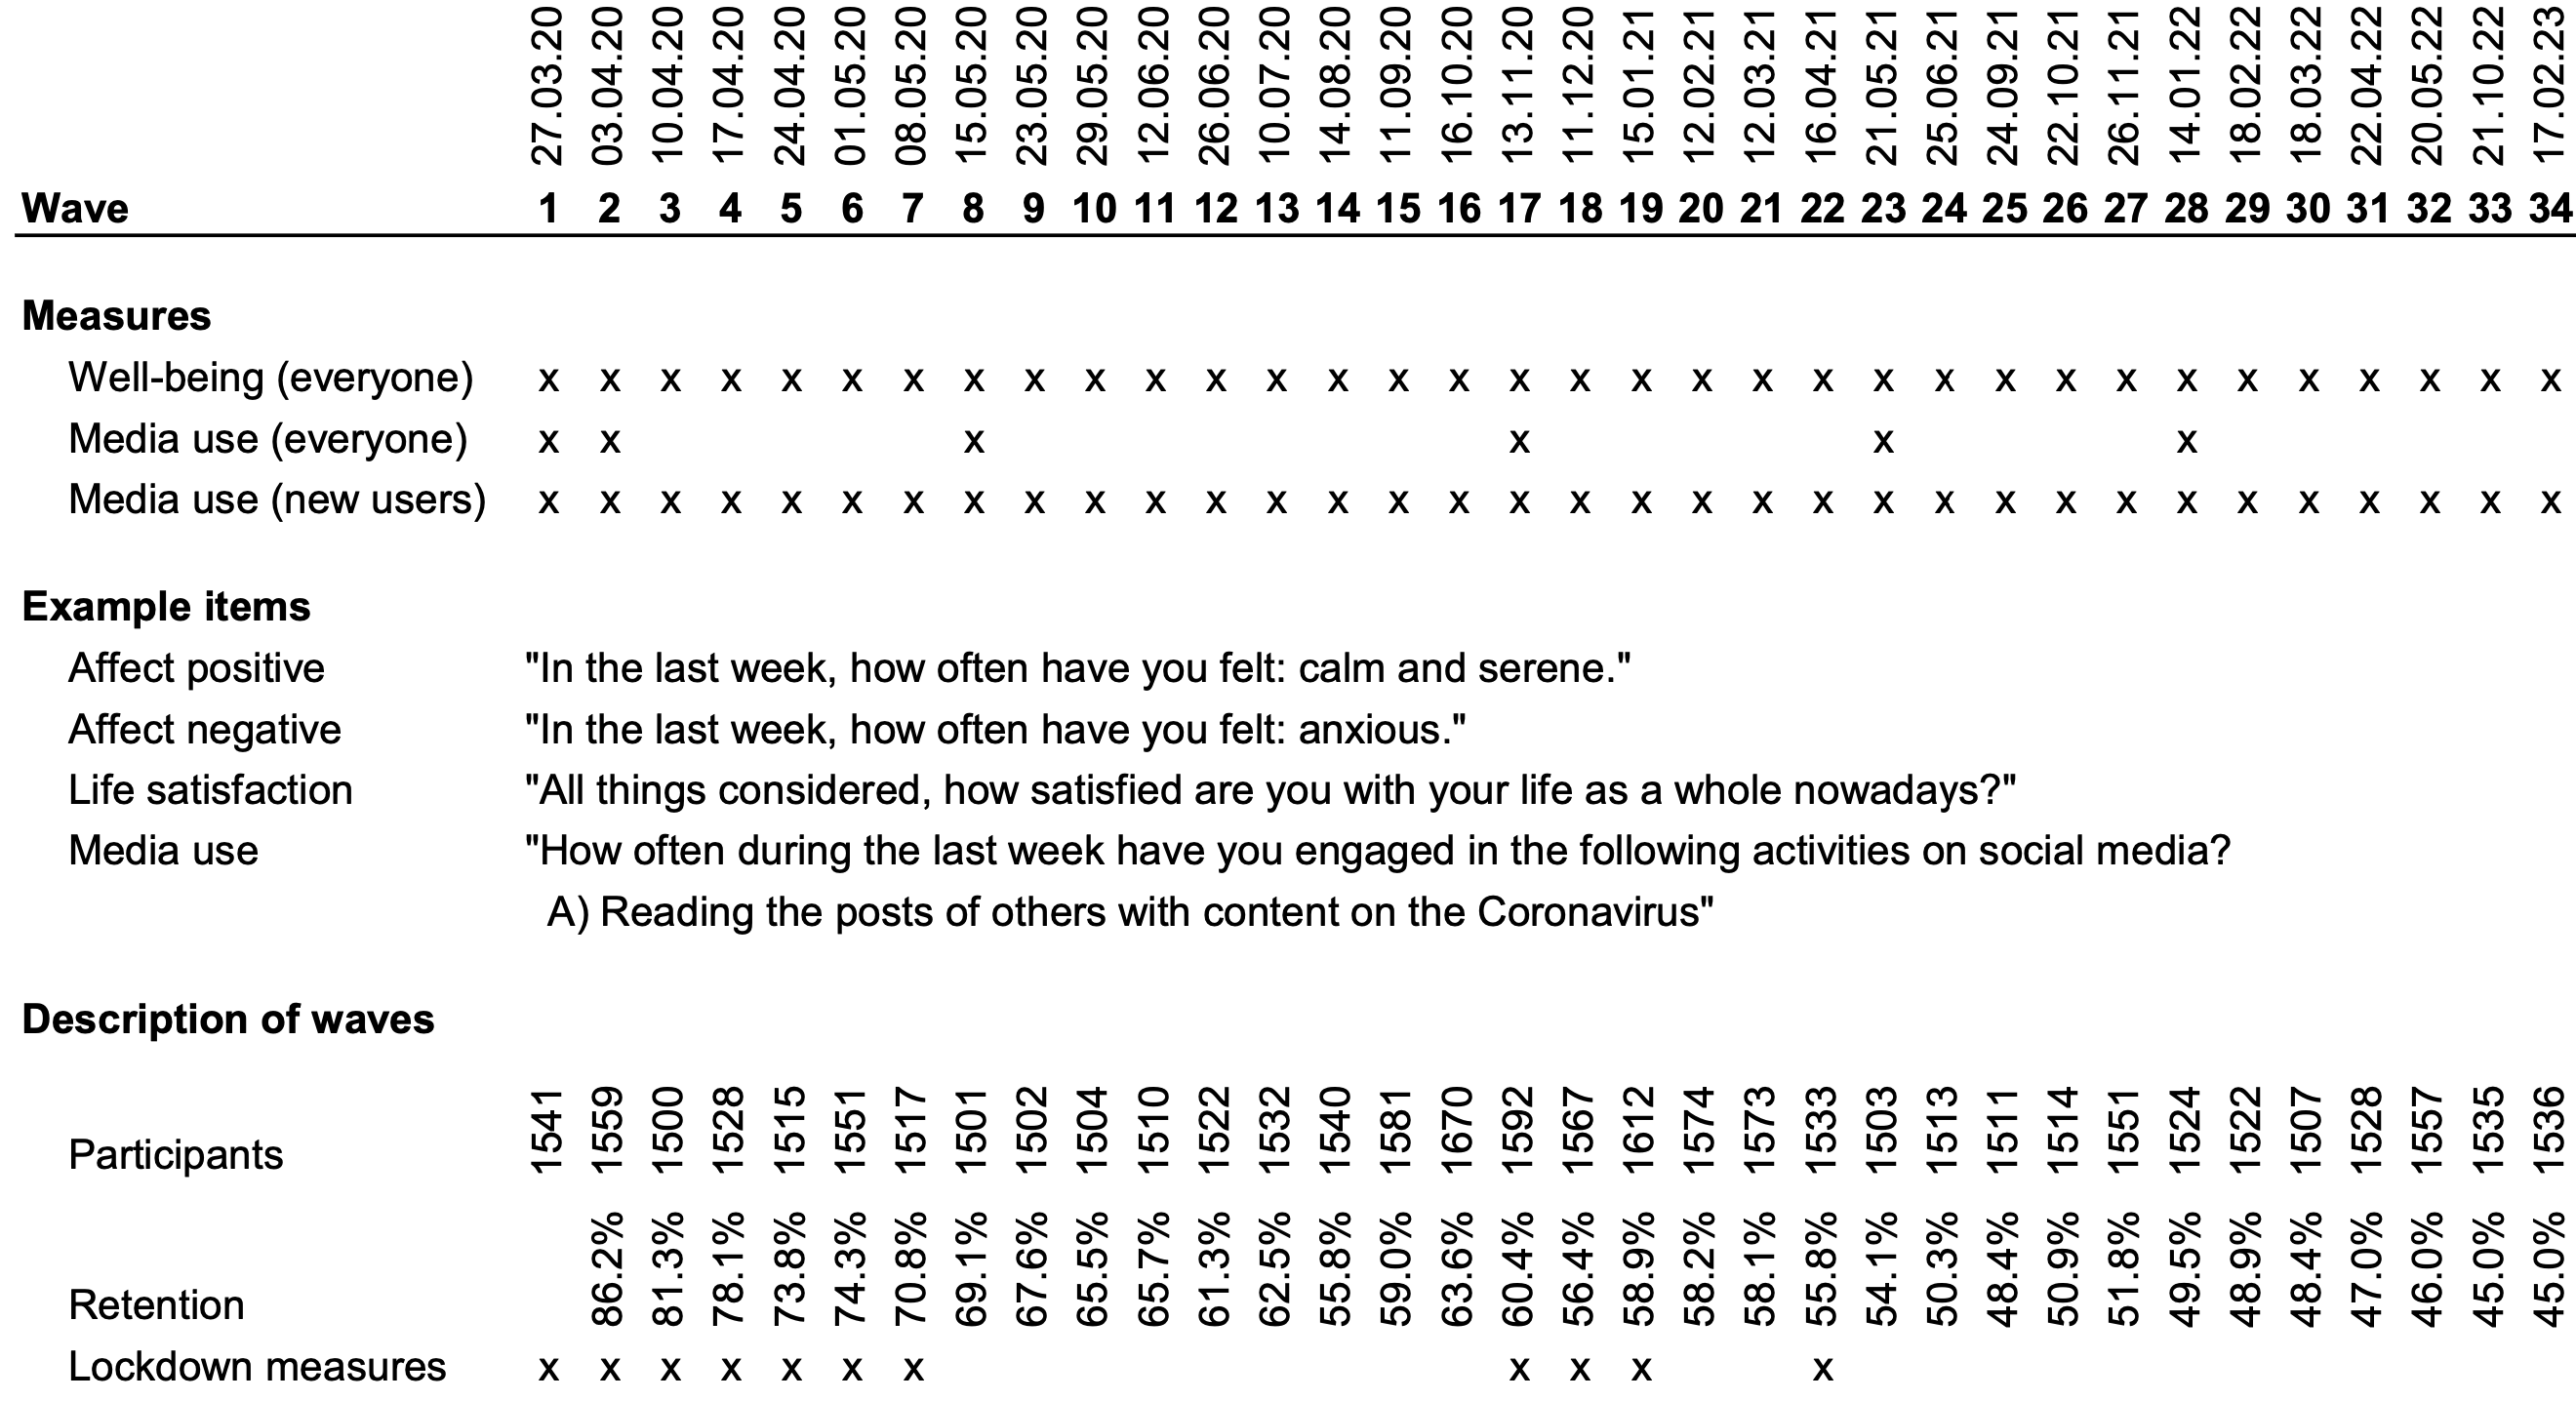
\includegraphics[width=1\textwidth]{figures/fig_study_description} \caption{Overview of study set-up}\label{fig:study-desc}
\end{figure}

Achieved via quota sampling, the sample matched the Austrian population in terms of age, gender, region/state, municipality size, and educational level.
In order to participate in the study, the respondents needed to be Austrian residents and had to be at least 14 years of age.
All respondents needed to have access to the internet (via computer or mobile devices such as smartphones or tablets).
Ethical review and approval was not required for the study in accordance with the local legislation and institutional requirements.
The participants provided their written informed consent to participate in this study.
The average age was 40 years, 49 percent were male, 14 percent had a University degree, and 5 percent were currently unemployed.

\hypertarget{smallest-effect-size-of-interest}{%
\subsection{Smallest Effect Size of Interest}\label{smallest-effect-size-of-interest}}

Testing the hypothesis necessitates defining what is considered a ``trivial effect size''.
To this end, we need to define a so-called smallest effect size of interest (SESOI) (Lakens et al., 2018).
A trivial effect would then need to be smaller than the SESOI (see below).
What could be a minimally interesting, nontrivial effect?
Being a normative question, finding a clear, single, or unanimous answer is impossible.
However, it is still necessary and helpful to work toward a plausible benchmark.
I suggest the following SESOI for this research question:

\begin{quote}
SESOI: If a heavy user of COVID-19 related social media news suddenly \emph{stops} using social media altogether, this should have a \emph{noticeable} impact on their overall well-being.
\end{quote}

What does this mean practically and how can it be operationalized?
In this study, COVID-19 related social media use was measured on a 5-point scale, ranging from 1 = \emph{never} to 5 = \emph{several times a day}. Thus, a change of four units in social media use (e.g., a complete stop) should correspond to a noticeable change in well-being.
What is a noticeable change in well-being?
According to Norman et al. (2003), people can reliably distinguish seven levels of satisfaction with health.
So if satisfaction is measured on a 7-point scale, a four unit change in social media use should result in a one unit change in life satisfaction.

In this study, life satisfaction was measured on an 11-point scale.
If people can reliably differentiate 7 levels, this corresponds to 11 / 7 = 1.57 unit change on an 11-point scale.
Hence, a four-point change in media use (e.g., a complete stop) should result in a 1.57-point change in life satisfaction.
In a statistical regression analysis, \emph{b} estimates the change in the dependent variable if the independent variable increases by one point.
For life satisfaction, we would therefore define a SESOI of \emph{b} = 1.57 / 4 = 0.39.
For positive or negative affect, which was measured on a 5-point scale, our SESOI would be \emph{b} = 0.71 / 4 = 0.18.
Because we are agnostic as to whether the effects are positive or negative, the null region includes both negative and positive effects.
Finally, in order not to exaggerate precision and to be less conservative, these numbers are reduced to nearby thresholds.\footnote{Note that other researchers also decreased or recommended decreasing thresholds for effect sizes when analyzing within-person or cumulative effects (Beyens et al., 2021; Funder \& Ozer, 2019).}
Together, this leads to a null region ranging from \emph{b} = -.30 to \emph{b} = .30 for life satisfaction, and \emph{b} = -.15 to \emph{b} = .15 for positive and negative affect.

The hypothesis is analyzed using the interval testing approach as proposed by Dienes (2014).
To illustrate, let us consider the case of life satisfaction {[}SESOI: -.30 : +.30{]}.
If the 95\% confidence interval falls completely within the null-region (e.g., \emph{b} = -.05, {[}95\% CI: -.15, .05{]}), the hypothesis that the effect is trivial is supported.
If the confidence interval falls completely outside of the null-region (e.g., \emph{b} = -.40, {[}95\% CI: -.45, -.35{]}), the hypothesis is rejected and the existence of a meaningful negative effect is supported.
If the confidence interval and the null region overlap (e.g., \emph{b} = -.30, {[}95\% CI: -.35, -.25{]}), the hypothesis is not supported and the results are considered inconclusive, while a meaningful positive effect is rejected.
If the confidence interval exceeds both sides of the null region (e.g., \emph{b} = -.025, {[}95\% CI: -.40, .35{]}), the hypothesis is not supported and judgement is suspended.
For an illustration, see Figure \ref{fig:sesoi}.

\begin{figure}
\centering
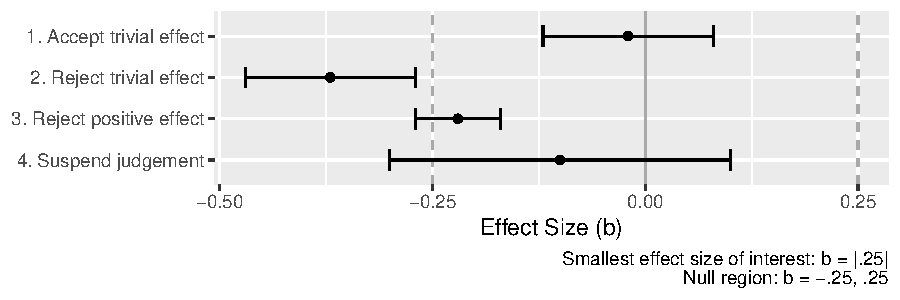
\includegraphics{manuscript_files/figure-latex/sesoi-1.pdf}
\caption{\label{fig:sesoi}Using confidence intervals to test a null region. In this study, a trivial effect of social media use on life satisfaction is defined as ranging from b = -.30 to b = .30. Figure adapted from Dienes (2014).}
\end{figure}

\hypertarget{data-analysis}{%
\subsection{Data Analysis}\label{data-analysis}}

\hypertarget{causality}{%
\subsubsection{Causality}\label{causality}}

When using longitudinal designs to analyze causality, it is important to (a) focus on within-person effects (Hamaker, 2014); to (b) control for confounders (Rohrer \& Murayama, 2023); and to (c) test a plausible interval between measures (Dormann \& Griffin, 2015).
First, in non-experimental designs it makes much sense to analyze causal effects from an internal, within-person perspective (Hamaker, 2014).
If a specific person changes their media diet, we need to measure how this behavior affects their well-being.
Between-person comparisons from longitudinal data cannot provide such insights (Hamaker, 2014).
To test the hypothesis, I thus consider only the within-person effects.

Second, to identify confounders we should control for variables that affect both media use and well-being, which helps isolate the actual effect (Rohrer, 2018).
Because we are adopting a within-person perspective, we need to implement \emph{time-varying} confounders (Rohrer \& Murayama, 2023).
And because we are determining the \emph{overall} causal effect, we need to make sure \emph{not} to control for mediating variables (Rohrer, 2018), for doing so would bias our assessment of the causal effect.
In this study, I hence preregistered to control for the following variables, which either have already been shown or are likely to affect both social media use and well-being, and which also are not mediators:
gender, age, education, Austria country of birth, Austria country of birth of parents, residency Vienna, text-based news consumption, video-based news consumption, household size, health, living space, access to garden, access to balcony, employment, work hours per week, being in home-office, household income, outdoor activities, disposition to take risks, and locus of control (Eger \& Maridal, 2015).

Finally, one precondition of causality is temporal order and finding a plausible interval (Dormann \& Griffin, 2015).
If variables are stable, longer intervals are needed; if they fluctuate, shorter intervals.
In the case of well-being, we need shorter intervals for the more fluctuating positive and negative affect, and longer ones for the more stable life satisfaction (Dienlin \& Johannes, 2020).
Whereas using social media can have instant effects on mood (Marciano et al., 2022), effects on life satisfaction often take longer to manifest.
For example, because media use leads to actual changes in specific behaviors, which then in turn affect life satisfaction (Dienlin et al., 2017).

In this study, I hence analyze how changes in using social media \emph{during the last week} affected changes in positive and negative affect \emph{during the same week}.
In other words, if people during the last week engaged in more COVID-19 related social media use than usual, did they feel better or worse during that week than usual?
For life satisfaction, I implemented a longer interval.
If people \emph{during the last week} used COVID-19 related social media more than they usually do, were they \emph{at the end of the week} more or less satisfied with their lives than they usually are?
This way it is analyzed if when a person changes their social media diet, are there (a) \emph{simultaneous} changes in their affect and (b) \emph{subsequent} changes in their life satisfaction?
For the main analyses, the interval is implemented via the wording of the items (see below), not by using lagged measures coming from prior waves waves.
In additional analyses, I also tested how media use affects well-being one month or four months later.
All analyses will be controlled for varying confounders (see below), which fosters a causal interpretation.

\hypertarget{statistical-model}{%
\subsubsection{Statistical model}\label{statistical-model}}

The hypothesis was analyzed using random effect within-between models (REWB, Bell et al., 2019).
Altogether three models were run, one for each dependent variable.
The data were hierarchical, and responses were separately nested in participants and waves (i.e., participants and waves were implemented as random effects).
Nesting in participants accounts for the longitudinal design.
Nesting in waves controls for general exogenous developments, such as general decreases in well-being in the population, for example due to lockdown measures.
Thus, there was no need additionally to control for specific phases or measures of the lockdown.
Predictors were modeled as fixed effects.
They included social media communication types and channels, separated into within and between-person factors, as well as stable and varying covariates.
Between-person predictors are the predictors centered on the grand mean; within-person predictors are the predictors centered on the person's mean.
Between-person predictors (which, measuring relations, are not of particular interest in this study) represent how the mean of one respondent differs from the mean of all the other respondents.
The within-person predictors represent how much a person at one specific wave differs from their own mean.
For example, we could find that on Wave 3 a person used social media more than usual, while also experiencing more negative affect than usual.
All predictors were included simultaneously in each of the three models.

The factorial validity of the scales were tested with confirmatory factor analyses (CFA).
Because Mardia's test showed that the assumption of multivariate normality was violated, I used the more robust Satorra-Bentler scaled and mean-adjusted test statistic (MLM) as estimator.
Mean scores were used for positive and negative affect.
Missing responses were imputed using multiple imputation with predictive mean matching (five iterations, 30 data-sets), including categorical variables.
All variables were imputed except the social media use measures, as they were not collected on each wave.
All variables included in the analyses presented here were used to impute missing data.
For the main analyses, results were pooled across all thirty data-sets.

To contextualize the results, I conducted additional exploratory analyses.
I reran the analyses (a) with additional not-preregistered covariates such as trust in media or government, (b) without covariates, (c) with single imputation, and (d) without imputation.
For more information on the analyses, a complete documentation of the models and results, and all additional analyses, see \href{https://XMtRA.github.io/Austrian_Corona_Panel_Project}{companion website}.

\hypertarget{measures}{%
\subsection{Measures}\label{measures}}

For the variables' means, range, and variance, see Table \ref{tab:tab-descriptives}.
For a complete list of all items and item characteristics, see \href{https://XMtRA.github.io/Austrian_Corona_Panel_Project}{companion website}.

\hypertarget{well-being}{%
\subsubsection{Well-being}\label{well-being}}

Life satisfaction was measured with the item ``All things considered, how satisfied are you with your life as a whole nowadays?'', which comes from the European Social Survey.
The response options ranged from 0 (\emph{extremely dissatisfied}) to 10 (\emph{extremely satisfied}).

To capture positive affect, respondents were asked how often in the last week they felt (a) calm and relaxed, (b) happy, and (c) full of energy (World Health Organization, 1998).
The response options were 1 (\emph{never}), 2 (\emph{on some days}), 3 (\emph{several times per week}), 4 (\emph{almost every day}), and 5 (\emph{daily}).
The scale showed good factorial fit, \(\chi^2\)(66) = 69.42, \emph{p} = .363, CFI = 1.00, RMSEA \textless{} .01, 90\% CI {[}\textless{} .01, .02{]}, SRMR = .01.
Reliability was high, \(\omega\) = .85.

For negative affect, respondents were asked how often in the last week they felt (a) lonely, (b) aggravated, (c) so depressed, that nothing could lift you up, (d) very nervous, (e) anxious, and (h) glum and sad (World Health Organization, 1998).
The response options were 1 (\emph{never}), 2 (\emph{on some days}), 3 (\emph{several times per week}), 4 (\emph{almost every day}), and 5 (\emph{daily}).
The scale showed good factorial fit, \(\chi^2\)(471) = 4012.14, \emph{p} \textless{} .001, CFI = .98, RMSEA = .07, 90\% CI {[}.07, .08{]}, SRMR = .03.
Reliability was high, \(\omega\) = .91.

All three variables were measured on each wave.

\hypertarget{covid-19-related-social-media-use}{%
\subsubsection{COVID-19 related social media use}\label{covid-19-related-social-media-use}}

COVID-19 related social media use focused on communication types was measured with the three dimensions of (a) reading, (b) liking and sharing, and (c) posting.
The items come from Wagner et al. (2018) and were adapted for the context of this study.
The general introductory question was ``How often during the last week have you engaged in the following activities on social media?''.
The three items were ``Reading the posts of others with content on the Coronavirus'', ``When seeing posts on the Coronavirus, I clicked `like', `share' or `retweet'\,'', ``I myself wrote posts on the Coronavirus on social media.''
Answer options were 1 (\emph{several times per day}), 2 (\emph{daily}), 3 (\emph{several times per week}), 4 (\emph{weekly}), 5 (\emph{never}).
The items were inverted for the analyses.

COVID-19 related social media use focused on channels was measured with five variables from Wagner et al. (2018), adapted for this study.
The general introductory question was ``How often in the last week have you followed information related to the Corona-crisis on the following social media?''
The five items were (a) Facebook, (b) Twitter, (c) Instagram, (d) Youtube, and (e) WhatsApp.
Again, the answer options were 1 (\emph{several times per day}), 2 (\emph{daily}), 3 (\emph{several times per week}), 4 (\emph{weekly}), 5 (\emph{never}).
Again, the items were inverted for the analyses.

Social media use was measured for all participants on waves 1, 2, 8, 17, 23, and 28 (see Figure 1).
Freshly recruited respondents always answered all questions on COVID 19-related social media use.
Because new respondents always provided data on media use, it was possible to include these data into the analyses.
Hence, for the main analyses data from all 34 waves were used.
In the additional analyses I tested longer intervals, namely if changes in social media use were associated with changes in well-being either one month of four months later.
For these analyzes I used the predictors from waves 1, 2, 8, 17, 23, and 28, to see if they predicted changes in well-being either one month or four months later.

\begin{table}[tbp]

\begin{center}
\begin{threeparttable}

\caption{\label{tab:tab-descriptives}Descriptives of the main variables.}

\small{

\begin{tabular}{lllll}
\toprule
 & \multicolumn{1}{c}{sd} & \multicolumn{1}{c}{min} & \multicolumn{1}{c}{max} & \multicolumn{1}{c}{mean}\\
\midrule
Well-being &  &  &  & \\
\ \ \ Life satisfaction & 2.23 & 6.32 & 6.60 & 6.49\\
\ \ \ Positive affect & 0.94 & 3.09 & 3.22 & 3.16\\
\ \ \ Negative affect & 0.77 & 1.75 & 1.86 & 1.81\\
Social media use &  &  &  & \\
\ \ \ Read & 1.38 & 1.92 & 2.88 & 2.35\\
\ \ \ Like \& share & 1.19 & 1.54 & 1.94 & 1.74\\
\ \ \ Posting & 0.89 & 1.36 & 1.42 & 1.40\\
Social media channel &  &  &  & \\
\ \ \ Facebook & 1.58 & 2.02 & 2.72 & 2.37\\
\ \ \ Twitter & 0.95 & 1.36 & 1.43 & 1.39\\
\ \ \ Instagram & 1.34 & 2.00 & 2.08 & 2.05\\
\ \ \ WhatsApp & 1.66 & 2.27 & 2.60 & 2.46\\
\ \ \ YouTube & 1.28 & 1.91 & 1.98 & 1.95\\
\bottomrule
\end{tabular}

}

\end{threeparttable}
\end{center}

\end{table}

\hypertarget{control-variables}{%
\subsubsection{Control variables}\label{control-variables}}

The effects of COVID-19 related social media use were controlled for the following stable variables:
gender (female, male, diverse), age, education (ten options), Austria country of birth (yes/no), Austria parents' country of birth (no parent, one parent, both parents), and household size.
I also controlled for the following varying covariates: five items on current living conditions, including self-reported physical health, whether participants contracted COVID-19 since the last wave, current household income, working in home-office, and overall work hours; nine items measuring use of specific national text-based and video-based news outlets; five items measuring outdoor activities such as exercise or meeting friends; and two more psychological measures including locus of control and disposition to take risks.

\hypertarget{results}{%
\section{Results}\label{results}}

\hypertarget{descriptive-analyses}{%
\subsection{Descriptive Analyses}\label{descriptive-analyses}}

Looking at the variables from a descriptive perspective, aligned with set-point theory we can see that the level of all well-being measures were surprisingly stable during data collection (see Figure \ref{fig:fig-descriptives}).
COVID-19 related social media use, however, showed changes.
Reading, sharing and liking COVID-19 related content decreased substantially (almost one scale point from 3 to 2).
Posting about COVID-19 related content stayed the same.
Using Facebook and WhatsApp for COVID-19 related content decreased.
Instagram, YouTube, and Twitter stayed the same.
The general initial decrease could be explained by the fact that the collection of data began at the end of March 2020, hence approximately three months after the pandemic's onset.
After an initial uptick, COVID-19 related social media use might have already been declining at the time.

\begin{figure}
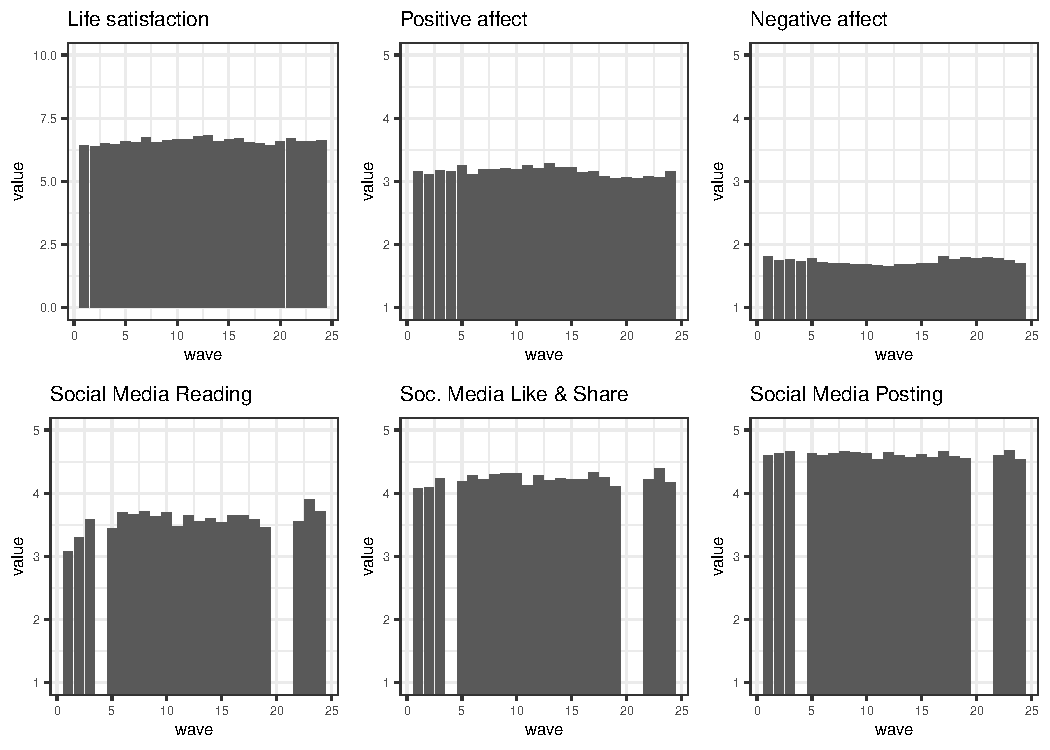
\includegraphics[width=\textwidth]{figures/fig_descriptives} \caption{Well-being and media use across the 34 waves. Note. Values obtained from mixed effect models, with participants and waves as grouping factors and without additional predictors.}\label{fig:fig-descriptives}
\end{figure}

Using the average values across all waves, which provides a stable picture of the general relations, I next looked at the correlations between social media use and well-being (see Figure \ref{fig:fig-correlations}).
Several interesting patterns emerged.
In general, people who spend more time engaging with COVID-19 related content on social media reported reduced well-being.
Users who spend more time reading, liking and sharing, and posting COVID-19 related content were less satisfied with their lives.
They also showed slightly less positive affect.
This overall negative picture was even more pronounced for negative affect.
People who engaged more with COVID-19 related content, including all types and channels of communication, reported substantially higher levels of negative affect.
For example, people who were more likely to post COVID-19 content had much higher levels of negative affect (\emph{r} = .61).
Note that these results represent between-person correlations, not causal within-person effects.

\begin{figure}
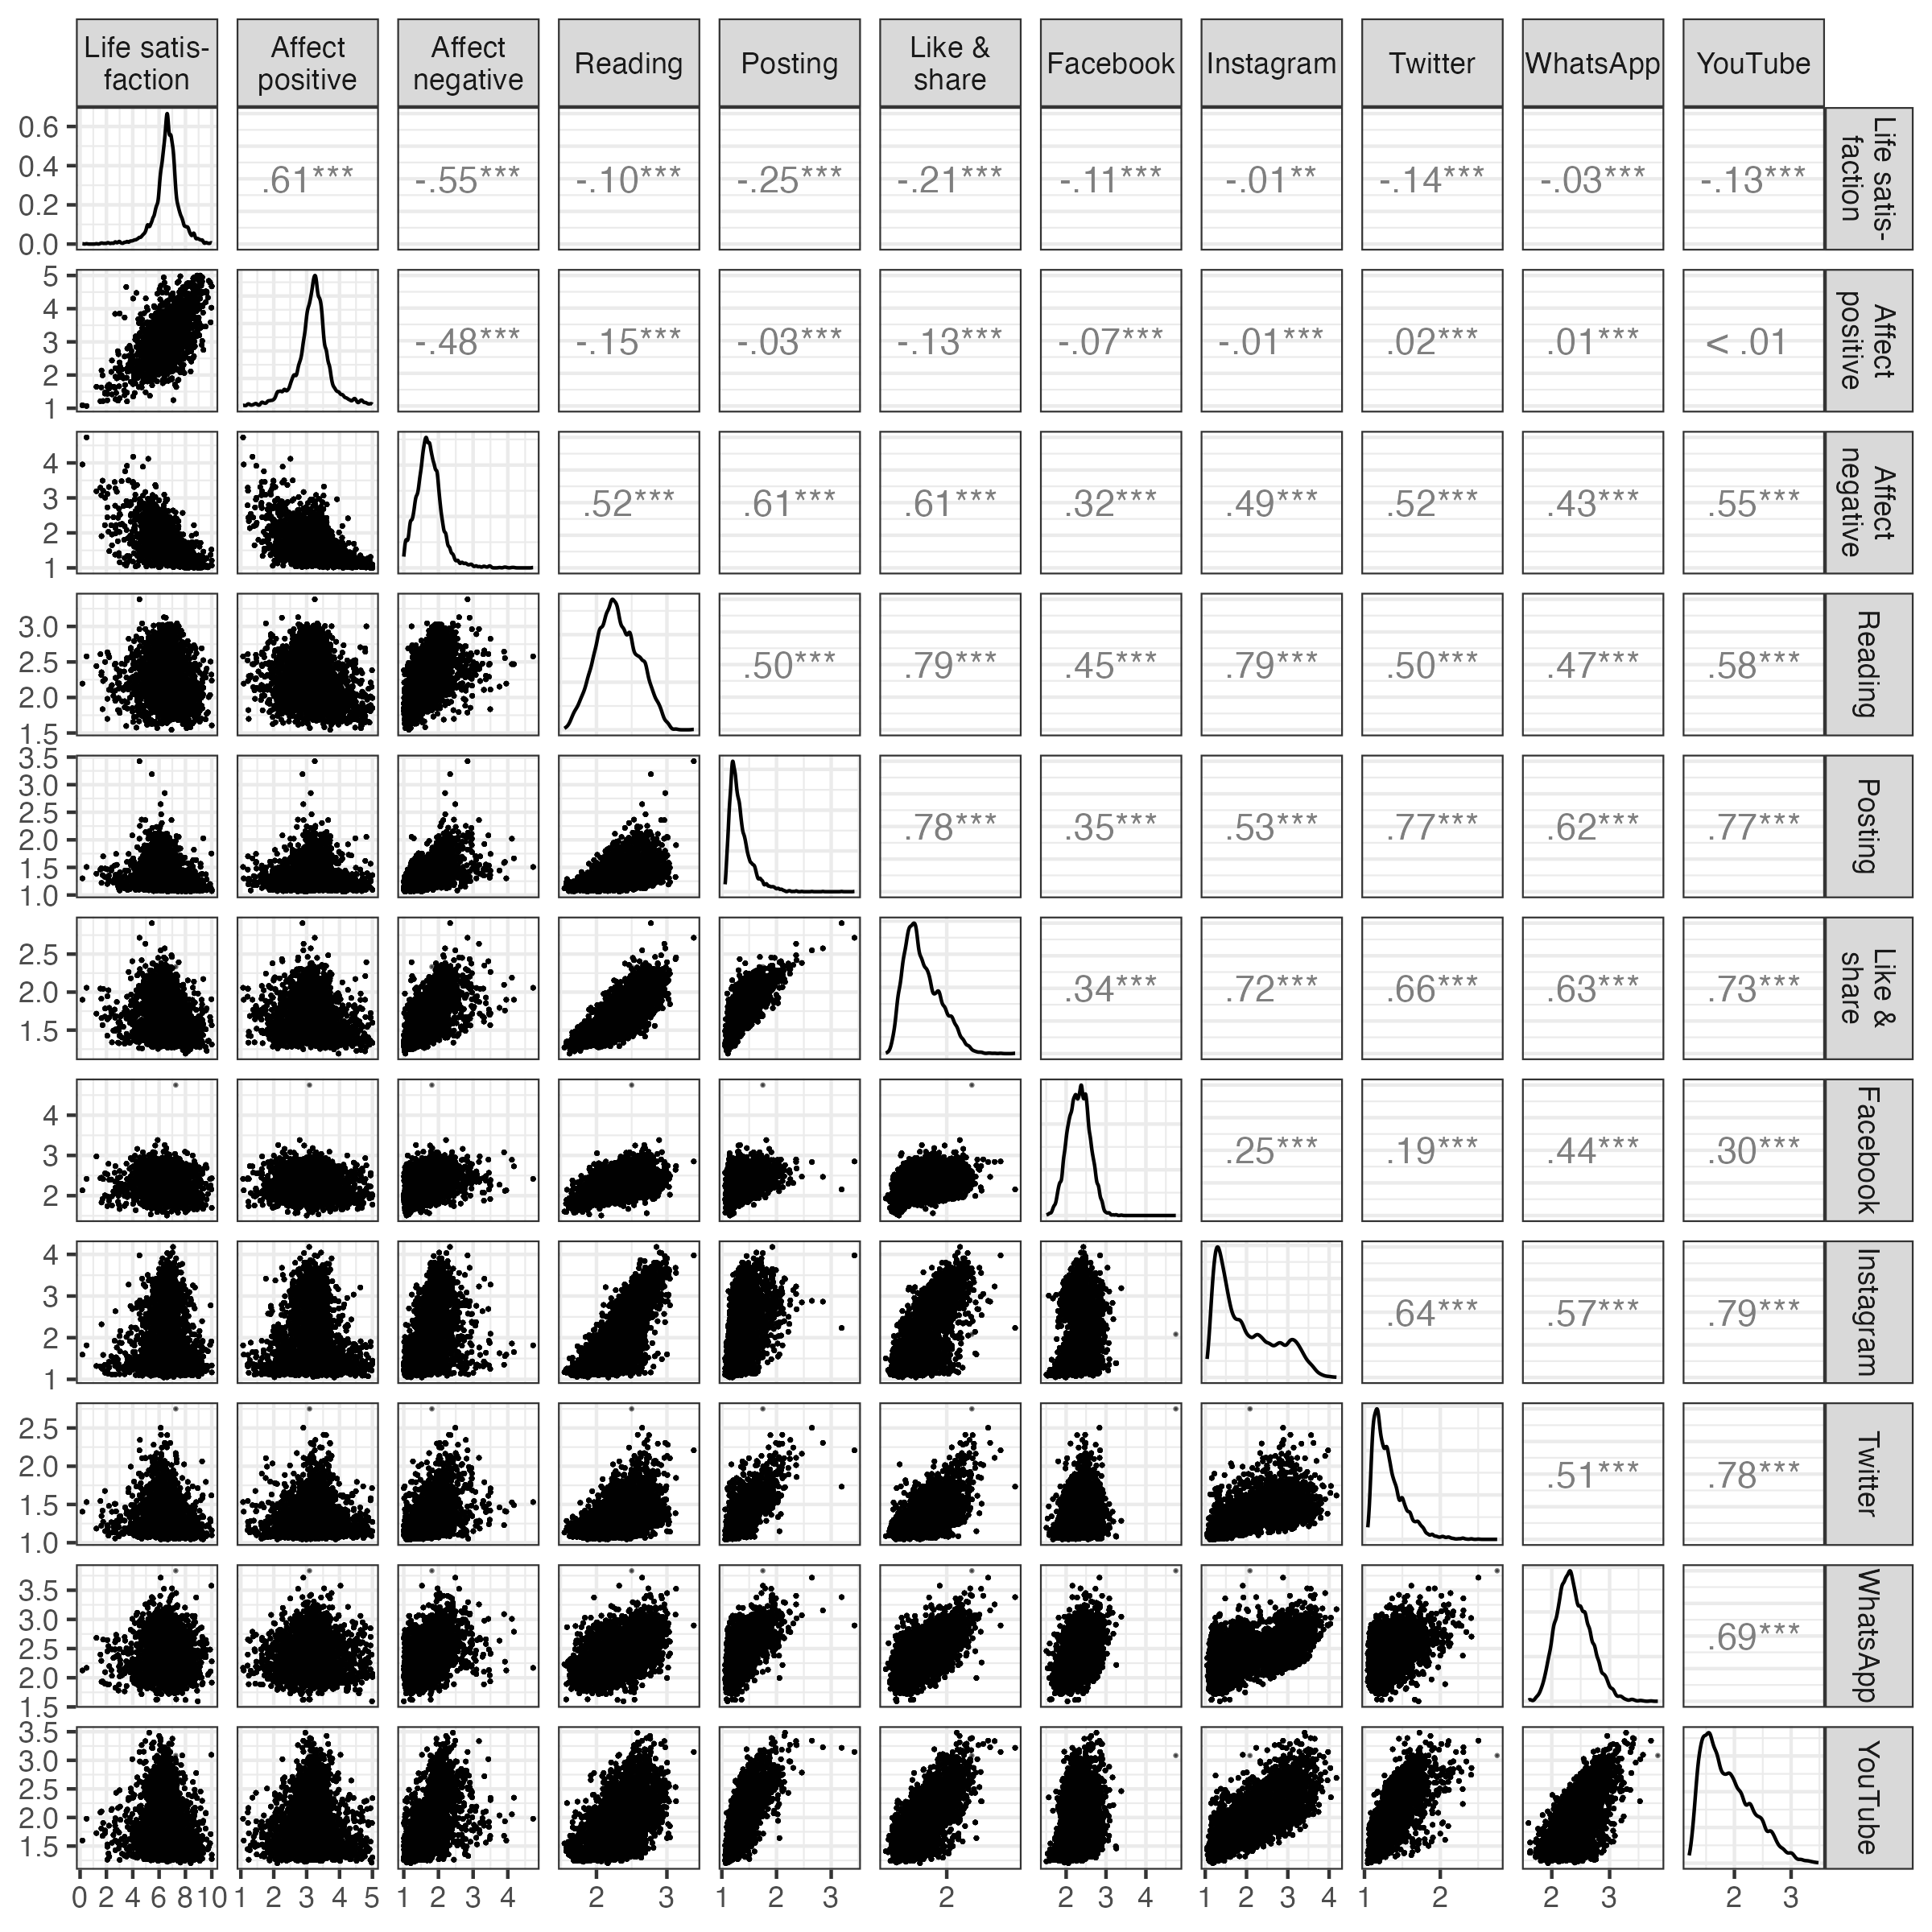
\includegraphics[width=\textwidth]{figures/fig_cor} \caption{Descriptives of the main variables, capturing well-being and social media use with their average values across all waves. Upper triangle: correlation coefficients; diagonal: density plots; lower triangle: scatter plots.}\label{fig:fig-correlations}
\end{figure}

\hypertarget{preregistered-analyses}{%
\subsection{Preregistered Analyses}\label{preregistered-analyses}}

\hypertarget{social-media-communication-types}{%
\subsubsection{Social media communication types}\label{social-media-communication-types}}

The study's main hypothesis was that the causal effects of all types and channels of social media use on all facets of well-being would be trivial.
Regarding the effects of different communication types (i.e., reading, sharing, of posting about COVID-19 related content), all within-person effects fell completely within the a-priori defined null region (see Figure \ref{fig:fig-within}).
For example, respondents who used social media more frequently than usual to like or share COVID-19 related content did not show a simultaneous change in life satisfaction (\emph{b} = -0.02 {[}95\% CI -0.06, 0.01{]}).
As a result, the hypothesis of trivial effects was supported for all COVID-19 related types of social media communication.

However, several effects stood out, as statistically they were significantly different from zero.
Users who read more COVID-19 related content than usual reported slightly reduced levels of positive affect (\emph{b} = -0.03 {[}95\% CI -0.05, -0.02{]}).
Users who liked and shared more COVID-19 related content than usual also experienced slightly more negative affect than usual (\emph{b} = 0.05 {[}95\% CI 0.04, 0.07{]}).
Posting COVID-19 related content affected all types of well-being.
Users who wrote more COVID-19 related posts than usual also reported slightly less life satisfaction than usual (\emph{b} = -0.04 {[}95\% CI -0.08, -0.01{]}) and slightly more negative affect than usual (\emph{b} = 0.05 {[}95\% CI 0.04, 0.07{]}).
Interestingly, however, users who wrote more COVID-19 related posts than usual also experienced slightly \emph{higher} levels of positive affect than usual (\emph{b} = 0.02 {[}95\% CI 0.01, 0.04{]}).

\hypertarget{social-media-communication-channels}{%
\subsubsection{Social media communication channels}\label{social-media-communication-channels}}

Regarding the COVID-19 related use of social media channels (i.e., Facebook, Instagram, WhatsApp, YouTube, and Twitter) the results were comparable (see Figure \ref{fig:fig-within}).
Changes in the frequency of using different social media channels to attain information regarding COVID-19 were unrelated to meaningful changes in well-being.
For example, respondents who used Facebook more frequently than usual to learn about COVID-19 did not show a simultaneous change in life satisfaction (\emph{b} -0.01 {[}95\% CI -0.04, 0.02{]}).
In sum, the hypothesis of trivial effects was supported also for the COVID-19 related use of important social media channels.

That said, two effects differed statistically from zero.
Respondents who used Twitter more frequently than usual to attain COVID-19 related news reported slightly higher levels of negative affect than usual (\emph{b} = 0.02 {[}95\% CI 0.01, 0.04{]}).
Likewise, respondents who used YouTube more frequently than usual for COVID-19 related issues reported slightly higher levels of negative affect than usual (\emph{b} = 0.01 {[}95\% CI \textless{} 0.01, 0.02{]}).
However, both effects were still completely inside of the null region, hence likely not large enough to be considered meaningful.

For an overview of all within-person effects, see Table \ref{tab:tab-within} and Figure \ref{fig:fig-within}.

\begin{figure}
\centering
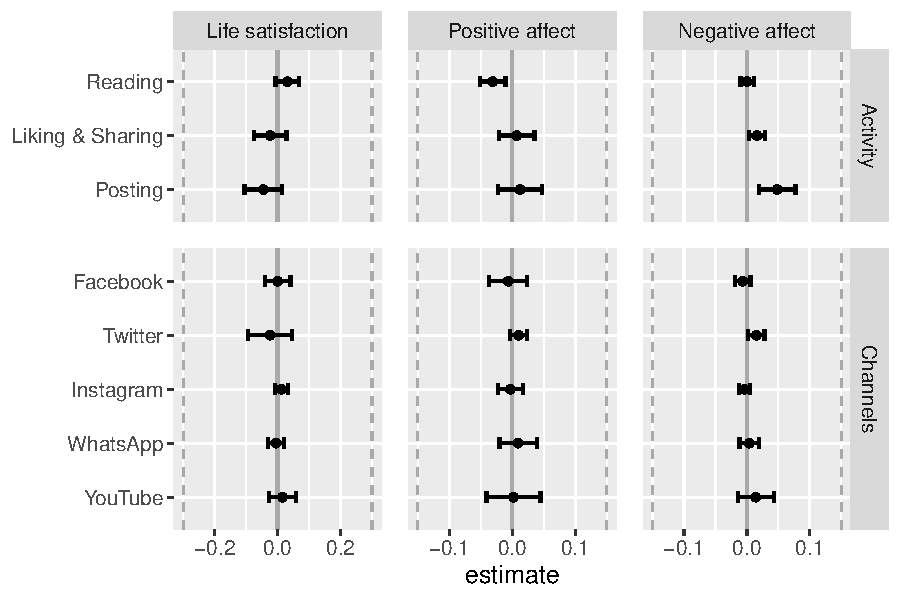
\includegraphics{manuscript_files/figure-latex/fig-within-1.pdf}
\caption{\label{fig:fig-within}Unstandardized within-person effects of COVID-19 related social media use on well-being. Note. The SESOI was b = \textbar0.30\textbar{} for life satisfaction and b = \textbar0.15\textbar{} for affect. Hence, all of the reported effects are not considered large enough to be meaningful.}
\end{figure}

\begin{table}[tbp]

\begin{center}
\begin{threeparttable}

\caption{\label{tab:tab-within}Overview of all within-person effects.}

\footnotesize{

\begin{tabular}{lrrrrr}
\toprule
 &  & \multicolumn{2}{c}{Confidence interval}  &  &\\
\cmidrule(r){3-4}
Predictor & \multicolumn{1}{c}{b} & \multicolumn{1}{c}{Lower} & \multicolumn{1}{c}{Higher} & \multicolumn{1}{c}{beta} & \multicolumn{1}{c}{p}\\
\midrule
Life satisfaction &  &  &  &  & \\
\ \ \ Reading & 0.01 & -0.03 & 0.05 & 0.01 & .639\\
\ \ \ Liking \& Sharing & -0.02 & -0.06 & 0.01 & -0.01 & .227\\
\ \ \ Posting & -0.04 & -0.08 & -0.01 & -0.02 & .025\\
\ \ \ Facebook & -0.01 & -0.04 & 0.02 & -0.01 & .527\\
\ \ \ Instagram & 0.03 & -0.01 & 0.07 & 0.02 & .149\\
\ \ \ WhatsApp & 0.00 & -0.04 & 0.04 & 0.00 & .917\\
\ \ \ YouTube & 0.01 & -0.03 & 0.04 & 0.00 & .713\\
\ \ \ Twitter & -0.01 & -0.05 & 0.03 & 0.00 & .503\\
Positive affect &  &  &  &  & \\
\ \ \ Reading & -0.03 & -0.05 & -0.02 & -0.04 & < .001\\
\ \ \ Liking \& Sharing & 0.01 & -0.01 & 0.02 & 0.01 & .508\\
\ \ \ Posting & 0.02 & 0.01 & 0.04 & 0.02 & .003\\
\ \ \ Facebook & 0.00 & -0.02 & 0.01 & 0.00 & .671\\
\ \ \ Instagram & -0.01 & -0.02 & 0.01 & -0.01 & .390\\
\ \ \ WhatsApp & 0.01 & -0.01 & 0.02 & 0.01 & .374\\
\ \ \ YouTube & 0.00 & -0.01 & 0.02 & 0.00 & .686\\
\ \ \ Twitter & 0.01 & 0.00 & 0.03 & 0.01 & .130\\
Negative affect &  &  &  &  & \\
\ \ \ Reading & 0.00 & -0.01 & 0.02 & 0.00 & .747\\
\ \ \ Liking \& Sharing & 0.02 & 0.00 & 0.04 & 0.02 & .022\\
\ \ \ Posting & 0.05 & 0.04 & 0.07 & 0.05 & < .001\\
\ \ \ Facebook & 0.00 & -0.01 & 0.01 & 0.00 & .710\\
\ \ \ Instagram & 0.00 & -0.02 & 0.01 & 0.00 & .654\\
\ \ \ WhatsApp & 0.00 & -0.01 & 0.01 & 0.01 & .417\\
\ \ \ YouTube & 0.01 & 0.00 & 0.02 & 0.02 & .011\\
\ \ \ Twitter & 0.02 & 0.01 & 0.04 & 0.02 & .008\\
\bottomrule
\end{tabular}

}

\end{threeparttable}
\end{center}

\end{table}

\hypertarget{exploratory-analyses}{%
\subsection{Exploratory Analyses}\label{exploratory-analyses}}

To contextualize the results reported above and to see if the study included any meaningful effects at all, I also looked at the effect sizes of the covariates.
Because each variable featured different response options, which would require defining a SESOI for each variable, I hence report the results of the standardized scales, which allows for a better comparison across the differently scaled variables.
Here, we can build on Cohen's convention that small effects begin at \emph{r} = \textbar.10\textbar.

The results showed that several effects crossed or fell completely outside of the SESOI, and can hence be considered meaningful.
For example, if physical health decreased, this had a meaningful detrimental impact on life satisfaction (\(\beta\) = .19 {[}95\% CI .18, .20{]}), positive affect (\(\beta\) = .18 {[}95\% CI .17, .19{]}), and negative affect (\(\beta\) = -.19 {[}95\% CI -.20, -.18{]}).
Spending more time outside to exercise meaningfully increased positive affect (\(\beta\) = .12 {[}95\% CI .11, .14{]}).
The strongest aspect affecting well-being was internal locus of control.
If people felt more in control of their lives, this strongly increased both life satisfaction (\(\beta\) = .33 {[}95\% CI .31, .35{]}) and
positive affect (\(\beta\) = .28 {[}95\% CI .27, .30{]}),
while decreasing negative affect (\(\beta\) = -.29 {[}95\% CI -.31, -.27{]}).
For an overview, see Figure \ref{fig:fig-control}.

\begin{figure}
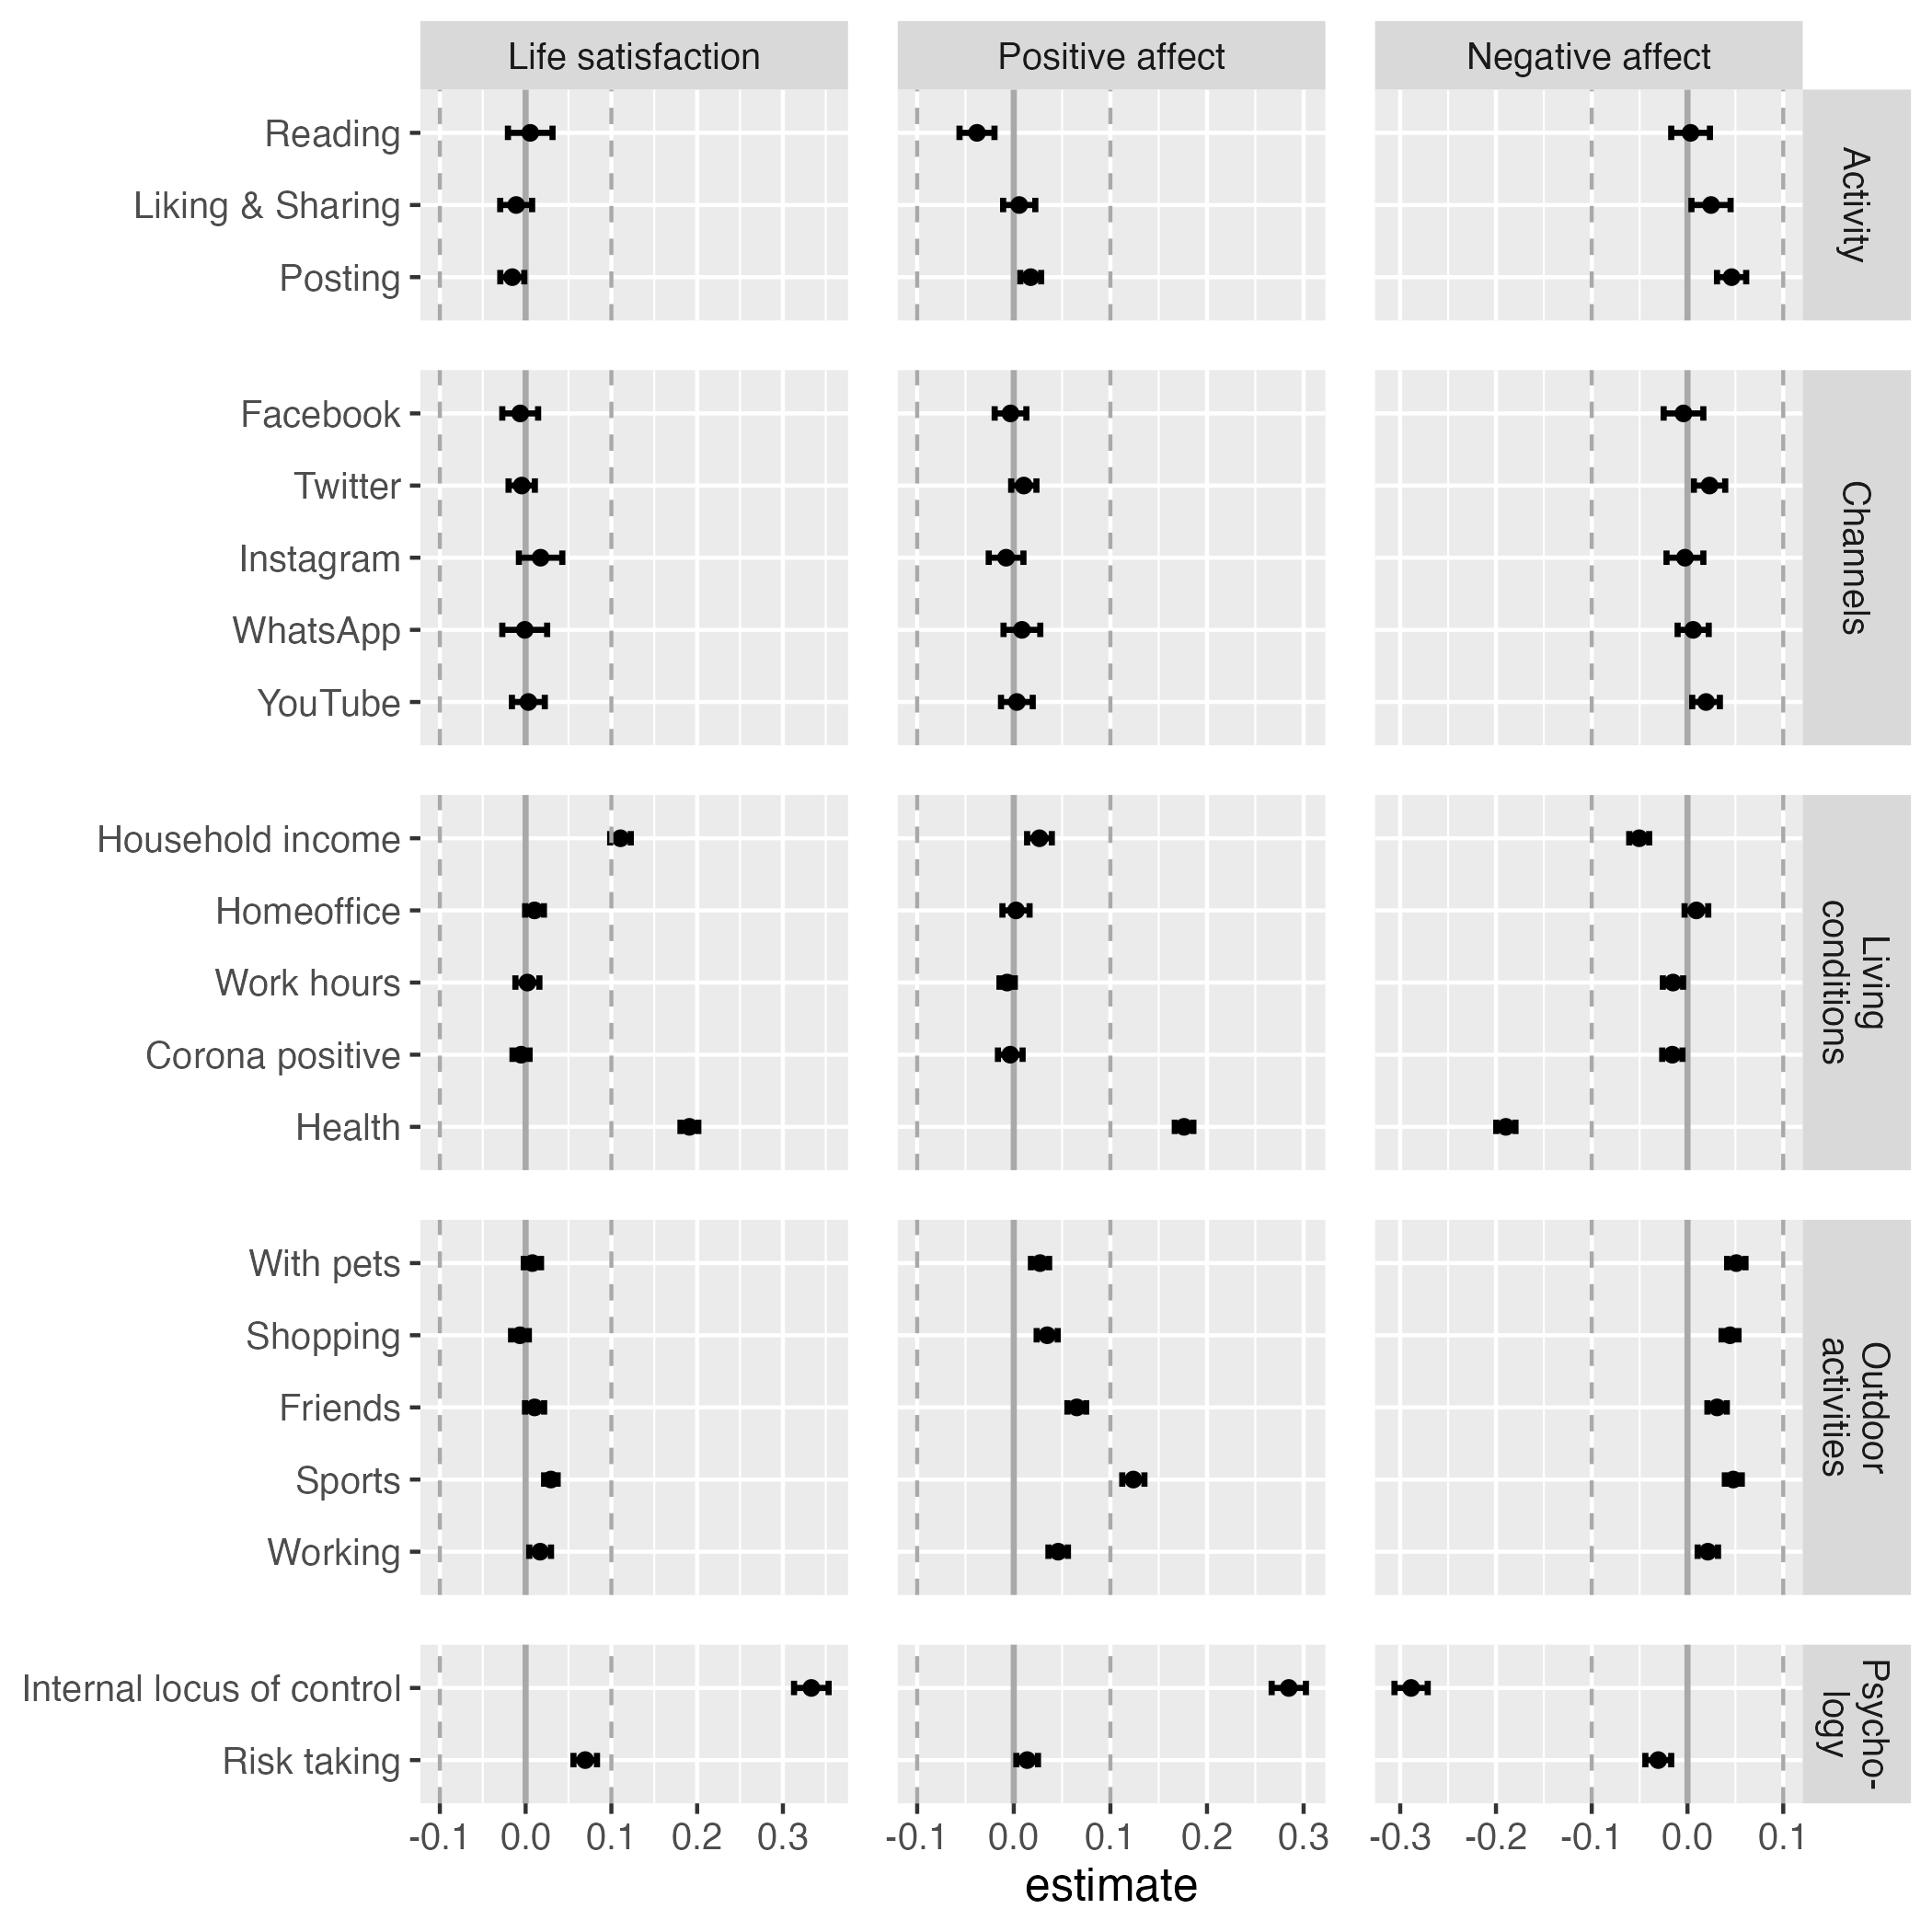
\includegraphics[width=\textwidth]{figures/fig_results_comp_std} \caption{Results of main variables together with covariates to provide context. All variables standardized. SESOI: beta = |.10|}\label{fig:fig-control}
\end{figure}

Because life satisfaction is more stable than affect, the effects of communication might materialize some time later.
I hence also tested the effects across the longer intervals of one month and four months.
Results showed that all effects disappeared.
No effect remained significant, implying that at least in this case in this case effects take place on a shorter interval.

Finally, as suggested by the differential susceptibility of media effects model, media effects can depend on dispositional factors, developmental stages, or cultural norms (Valkenburg \& Peter, 2013), such as gender and age (Orben et al., 2022).
I hence reran the analyses, differentiating effects for boys and girls and for age cohorts.
The results showed that effects did not differ across genders.
The effects also did not depend on age.
However, one effect stood out and was significant.
Compared to the middle age category Generation X, results showed that if users from Generation Z posted more COVID-19 content than usual this lead to significantly more negative affect (\(\beta\) = .04 {[}95\% CI .01, .06{]}).

\hypertarget{discussion}{%
\section{Discussion}\label{discussion}}

Based on a panel study with 34 waves largely representative of the Austrian population, this study analyzed the effects of COVID-19 related social media use on well-being.
Between person correlation analyses showed that more active users of COVID-19 related content on social media also reported decreased well-being.
For example, respondents who read more COVID-19 related content than others reported slightly lower levels of life satisfaction, somewhat lower levels of positive affect, and substantially higher levels of negative affect than others.
To see if these between person correlations would translate to within-person effects, I analyzed if changes in a person's media use led to changes in their well-being.
The within-person relations showed a different pattern.
If people consumed more COVID-19 content on social media than usual, this did not meaningfully reduce their well-being.
Although several statistically significant effects were found, these were very small.
For example, people who read more COVID-19 related posts than usual reported slightly decreased positive affect.
People who liked and shared more COVID-19 related posts than usual reported slightly higher levels of negative affect.
Posting more content about COVID-19 than usual slightly decreased life satisfaction, while increasing both negative affect and positive affect.
Using Twitter for COVID-19 related content slightly increased negative affect, as did YouTube.
Again, although all of these within-person effects were statistically significant, they were very small, smaller than the predefined smallest effect size of interest.
According to the preregistered procedure, they should hence be considered irrelevant.
Additional analyses revealed that other factors, for which we would expect to find meaningful effects, such as health or sports, indeed showed substantial and meaningful impacts on well-being.
In addition, when testing for the longer intervals of one month and four months, again no meaningful effects were found.
In conclusion, COVID-19 related activity on social media was not a particularly strong influence on peoples' well-being.
The results do not support the popular fears that ``doomscrolling'' or overusing social media during times of crises constitutes a prominent risk for well-being.

These specific observations notwithstanding, several general trends can be observed.
First, overall the results do suggest that effects of COVID-19 related social media use on well-being tend to take place in the negative as opposed to the positive spectrum.
Although very small, five statistically significant negative results of COVID-19 related social media use on well-being were found.
Only one positive effect emerged.

Second, six significant outcomes emerged for positive or negative affect, but only one for life satisfaction.
Life satisfaction is more stable and not that easily affected by any type or channel of social media communication.
The more fluctuating positive and negative affect, however, were affected (albeit only slightly).
Liking, sharing, and posting COVID-19 related content, and spending more time on Twitter and YouTube to browse COVID-19 related content, all slightly negatively influenced affect.
This is aligned with prior findings which showed that social media use is associated with increased negative affect but not with life satisfaction (Meier \& Reinecke, 2020).
Conversations about COVID-19 on social media are often extreme, negative, or aggressive (L. Fan et al., 2020).
More deeply engaging with this type of content could negatively affect active authors.
The hypothesis that tonality could explain the negative effects is especially supported by the observation that spending more time on Twitter and YouTube than usual increased negative affect.
Communication on both channels is often found to be negative and impolite (e.g., Mueller \& Saeltzer, 2022).
Consuming more negative and misleading information could hence explain the (slightly) increased levels of negative affect.

Third, the results show that it makes sense to analyze different communication types and communication channels.
Reading slightly reduced positive affect, while liking, sharing, and posting slightly increased negative affect.
Interestingly, posting COVID-19 related comment slightly increased negative affect, while at the same time it also slightly increased positive affect.
Posting content is often met with strong reaction, both positive by means of likes and negative by means of critical comments.
Overall, though, posting led to slightly reduced levels of life satisfaction.
In conclusion, whereas it was often stated that passive use is bad and active use good (Verduyn et al., 2015), this pattern was only partially found here.
The results are aligned with the findings from Valkenburg et al. (2022), who could not confirm that active use is good and that passive use is bad.
Focusing on communication channels, Twitter and YouTube seem to be more negative, while Instagram, WhatsApp, and Facebook were neutral.
But, again, all of these effects are very small.

Taken together, the results are hence aligned with the underlying theoretical models and prior empirical results.
The findings support the differential susceptibility of media effects model (Valkenburg \& Peter, 2013), such that effects are generally small and that they depend on the type and channel of communication.
Additional analyses did not reveal that effects depended on gender.
Age also large did not play a significant moderation role, but effects of posting COVID-19 related content were found to be more negative for Generation Z.
Indeed, it has often been argued that effects of social media use are more negative for Gen Z than for prior generations, and this finding can be seen a further tentative support for this hypothesis.
From a broader perspective, the results are well-aligned with mood management theory (Zillmann, 1988) and the uses and gratifications approach (Katz et al., 1973), whose premises preclude particularly negative effects of routine and widespread media consumption.
Both theories posit that if the effects of social media were indeed profoundly negative on average, then people likely would not spend so much time on social media engaging with COVID-19 content.
Finally, recent empirical studies and meta-analyses reported rather small negative effects, too (Meier \& Reinecke, 2020),
echoing the results obtained here.

\hypertarget{limitations}{%
\subsection{Limitations}\label{limitations}}

Focusing on within-person effects and controlling for several potential confounders, this study provides an improved perspective on assessing causality.
However, several challenges remain.
In order to correctly establish causality in non-experimental designs, it is necessary to control for \emph{all} relevant confounding third variables (Rohrer, 2018).
Although this study included are large list of confounders, it could still be that crucial variables were missed.
More thought needs to be invested in which factors to control for and, equally important, for which factors not to control for.

Although I had already reduced the predefined SESOIs to be less conservative, one could argue they were still too large.
Media use is only one aspect of several factors that simultaneously affect well-being.
Is it realistic to expect that changing only \emph{one} of these aspects should already manifest in a detectable change in well-being?
Or would it make more sense to expect that thoroughly committing to say \emph{two} activities (e.g.~regularly exercising \emph{and} establishing a reading habit) should then cause a detectable improvement in well-being?
Practically, this would imply a SESOI half the size defined here, namely \emph{b} = \textbar.15\textbar{} for life satisfaction and \emph{b} = \textbar.075\textbar{} for affect.
In the case of this study, however, even halving the SESOI would not make a difference.
All but one effect would still be completely in the null region, and no effect would fall completely outside of the null region.
I encourage future research to elaborate on what effect sizes are considered meaningful and what not.

Both media use and well-being were measured using self-reports.
Because assessing well-being necessarily requires introspection, using self-reports for affect and life satisfaction is adequate.
However, for social media use objective measures are preferable, as people often cannot reliably estimate their use (Scharkow, 2016).

Being collected in a single country, the generalizability of the results is limited.
They might not hold true in other cultures, especially non-Western cultures with a different media landscape or alternative social media channels.

\hypertarget{conclusion}{%
\subsection{Conclusion}\label{conclusion}}

In this study, COVID-19 related social media use did not meaningfully affect well-being.
Very small negative effects were found for writing COVID-19 related posts, sharing COVID-19 related content, and spending more time than usual on Twitter.
Factors other than social media use, however, were meaningfully related to well-being, including physical health, exercise, satisfaction with democracy, or believing that one is in control of one's life.
In light of the overall very small effects, engaging in COVID 19-related social media use should not be considered a major concern for one's well-being.

\newpage

\hypertarget{references}{%
\section{References}\label{references}}

\hypertarget{refs}{}
\begin{CSLReferences}{1}{0}
\leavevmode\vadjust pre{\hypertarget{ref-atheyDigitalPublicHealth2023}{}}%
Athey, S., Grabarz, K., Luca, M., \& Wernerfelt, N. (2023). Digital public health interventions at scale: {The} impact of social media advertising on beliefs and outcomes related to {COVID} vaccines. \emph{Proceedings of the National Academy of Sciences}, \emph{120}(5), e2208110120. \url{https://doi.org/10.1073/pnas.2208110120}

\leavevmode\vadjust pre{\hypertarget{ref-bellFixedRandomEffects2019}{}}%
Bell, A., Fairbrother, M., \& Jones, K. (2019). Fixed and random effects models: Making an informed choice. \emph{Quality \& Quantity}, \emph{53}(2), 1051--1074. \url{https://doi.org/10.1007/s11135-018-0802-x}

\leavevmode\vadjust pre{\hypertarget{ref-bendauAssociationsCOVID19Related2021}{}}%
Bendau, A., Petzold, M. B., Pyrkosch, L., Mascarell Maricic, L., Betzler, F., Rogoll, J., Große, J., Ströhle, A., \& Plag, J. (2021). Associations between {COVID-19} related media consumption and symptoms of anxiety, depression and {COVID-19} related fear in the general population in {Germany}. \emph{European Archives of Psychiatry and Clinical Neuroscience}, \emph{271}(2), 283--291. \url{https://doi.org/10.1007/s00406-020-01171-6}

\leavevmode\vadjust pre{\hypertarget{ref-beyensSocialMediaUse2021}{}}%
Beyens, I., Pouwels, J. L., van Driel, I. I., Keijsers, L., \& Valkenburg, P. M. (2021). Social media use and adolescents' well-being: {Developing} a typology of person-specific effect patterns. \emph{Communication Research}. \url{https://doi.org/10.1177/00936502211038196}

\leavevmode\vadjust pre{\hypertarget{ref-dienerAdvancesOpenQuestions2018}{}}%
Diener, E., Lucas, R. E., \& Oishi, S. (2018). Advances and open questions in the science of subjective well-being. \emph{Collabra: Psychology}, \emph{4}(1), 15. \url{https://doi.org/10.1525/collabra.115}

\leavevmode\vadjust pre{\hypertarget{ref-dienesUsingBayesGet2014}{}}%
Dienes, Z. (2014). Using {Bayes} to get the most out of non-significant results. \emph{Frontiers in Psychology}, \emph{5}. \url{https://doi.org/10.3389/fpsyg.2014.00781}

\leavevmode\vadjust pre{\hypertarget{ref-dienlinImpactDigitalTechnology2020}{}}%
Dienlin, T., \& Johannes, N. (2020). The impact of digital technology use on adolescent well-being. \emph{Dialogues in Clinical Neuroscience}, \emph{22}(2), 135--142. \url{https://doi.org/doi:10.31887/DCNS.2020.22.2/tdienlin}

\leavevmode\vadjust pre{\hypertarget{ref-dienlinDisplacementReinforcementReciprocity2017}{}}%
Dienlin, T., Masur, P. K., \& Trepte, S. (2017). Displacement or reinforcement? {The} reciprocity of {FtF}, {IM}, and {SNS} communication and their effects on loneliness and life satisfaction. \emph{Journal of Computer-Mediated Communication}, \emph{22}(2), 71--87. \url{https://doi.org/10.1111/jcc4.12183}

\leavevmode\vadjust pre{\hypertarget{ref-dormannOptimalTimeLags2015}{}}%
Dormann, C., \& Griffin, M. A. (2015). Optimal time lags in panel studies. \emph{Psychological Methods}, \emph{20}(4), 489--505. \url{https://doi.org/10.1037/met0000041}

\leavevmode\vadjust pre{\hypertarget{ref-edenMediaCopingCOVID192020}{}}%
Eden, A. L., Johnson, B. K., Reinecke, L., \& Grady, S. M. (2020). Media for coping during {COVID-19} social distancing: {Stress}, anxiety, and psychological well-being. \emph{Frontiers in Psychology}, \emph{11}, 577639. \url{https://doi.org/10.3389/fpsyg.2020.577639}

\leavevmode\vadjust pre{\hypertarget{ref-egerStatisticalMetaanalysisWellbeing2015}{}}%
Eger, R. J., \& Maridal, J. H. (2015). A statistical meta-analysis of the wellbeing literature. \emph{International Journal of Wellbeing}, \emph{5}(2), 45--74. \url{https://doi.org/10.5502/ijw.v5i2.4}

\leavevmode\vadjust pre{\hypertarget{ref-fanInformationOverloadWellbeing2021}{}}%
Fan, J., \& Smith, A. P. (2021). Information overload, wellbeing and {COVID-19}: {A} survey in {China}. \emph{Behavioral Sciences}, \emph{11}(5), 62. \url{https://doi.org/10.3390/bs11050062}

\leavevmode\vadjust pre{\hypertarget{ref-fanStigmatizationSocialMedia2020}{}}%
Fan, L., Yu, H., \& Yin, Z. (2020). Stigmatization in social media: {Documenting} and analyzing hate speech for {\textsc{COVID}} -19 on {Twitter}. \emph{Proceedings of the Association for Information Science and Technology}, \emph{57}(1). \url{https://doi.org/10.1002/pra2.313}

\leavevmode\vadjust pre{\hypertarget{ref-funderEvaluatingEffectSize2019}{}}%
Funder, D. C., \& Ozer, D. J. (2019). Evaluating effect size in psychological research: {Sense} and nonsense. \emph{Advances in Methods and Practices in Psychological Science}, \emph{2}(2), 156--168. \url{https://doi.org/10.1177/2515245919847202}

\leavevmode\vadjust pre{\hypertarget{ref-guazziniSecondWaveAnalysis2022}{}}%
Guazzini, A., Pesce, A., Marotta, L., \& Duradoni, M. (2022). Through the second wave: {Analysis} of the psychological and perceptive changes in the {Italian} population during the {COVID-19} pandemic. \emph{International Journal of Environmental Research and Public Health}, \emph{19}(3), 1635. \url{https://doi.org/10.3390/ijerph19031635}

\leavevmode\vadjust pre{\hypertarget{ref-hamakerWhyResearchersShould2014}{}}%
Hamaker, E. L. (2014). Why researchers should think "within-person": {A} paradigmatic rationale. In M. R. Mehl, T. S. Conner, \& M. Csikszentmihalyi (Eds.), \emph{Handbook of research methods for studying daily life} (Paperback ed.). {Guilford}.

\leavevmode\vadjust pre{\hypertarget{ref-huntSocialMediaBased2022}{}}%
Hunt, I. de V., Dunn, T., Mahoney, M., Chen, M., Nava, V., \& Linos, E. (2022). A social media-based public health campaign encouraging {COVID-19} vaccination across the {United States}. \emph{American Journal of Public Health}, \emph{112}(9), 1253--1256. \url{https://doi.org/10.2105/AJPH.2022.306934}

\leavevmode\vadjust pre{\hypertarget{ref-johnhopkinsuniversityCOVID19Map2023}{}}%
John Hopkins University. (2023). {COVID-19 Map}. In \emph{Johns Hopkins Coronavirus Resource Center}. https://coronavirus.jhu.edu/map.html.

\leavevmode\vadjust pre{\hypertarget{ref-katzUsesGratificationsResearch1973}{}}%
Katz, E., Blumler, J. G., \& Gurevitch, M. (1973). Uses and {Gratifications Research}. \emph{Public Opinion Quarterly}, \emph{37}(4), 509. \url{https://doi.org/10.1086/268109}

\leavevmode\vadjust pre{\hypertarget{ref-kittelAustrianCoronaPanel2020}{}}%
Kittel, B., Kritzinger, S., Boomgaarden, H., Prainsack, B., Eberl, J.-M., Kalleitner, F., Lebernegg, N. S., Partheymüller, J., Plescia, C., Schiestl, D. W., \& Schlogl, L. (2020). \emph{Austrian {Corona Panel Project} ({SUF} edition)}. {AUSSDA}. \url{https://doi.org/10.11587/28KQNS}

\leavevmode\vadjust pre{\hypertarget{ref-lakensEquivalenceTestingPsychological2018}{}}%
Lakens, D., Scheel, A. M., \& Isager, P. M. (2018). Equivalence testing for psychological research: {A} tutorial. \emph{Advances in Methods and Practices in Psychological Science}, \emph{1}(2), 259--269. \url{https://doi.org/10.1177/2515245918770963}

\leavevmode\vadjust pre{\hypertarget{ref-latikkaLonelinessPsychologicalDistress2022}{}}%
Latikka, R., Koivula, A., Oksa, R., Savela, N., \& Oksanen, A. (2022). Loneliness and psychological distress before and during the {COVID-19} pandemic: {Relationships} with social media identity bubbles. \emph{Social Science \& Medicine}, \emph{293}, 114674. \url{https://doi.org/10.1016/j.socscimed.2021.114674}

\leavevmode\vadjust pre{\hypertarget{ref-liYouTubeSourceInformation2020}{}}%
Li, H. O.-Y., Bailey, A., Huynh, D., \& Chan, J. (2020). {YouTube} as a source of information on {COVID-19}: A pandemic of misinformation? \emph{BMJ Global Health}, \emph{5}(5), e002604. \url{https://doi.org/10.1136/bmjgh-2020-002604}

\leavevmode\vadjust pre{\hypertarget{ref-lucasAdaptationSetpointModel2007}{}}%
Lucas, R. E. (2007). Adaptation and the set-point model of subjective well-being. \emph{Current Directions in Psychological Science}, \emph{16}(2), 75--79. \url{https://doi.org/10.1111/j.1467-8721.2007.00479.x}

\leavevmode\vadjust pre{\hypertarget{ref-lykkenHappinessWhatStudies1999}{}}%
Lykken, D. T. (1999). \emph{Happiness: {What} studies on twins show us about nature, nurture, and the happiness set-point}. {Golden Books}.

\leavevmode\vadjust pre{\hypertarget{ref-marcianoDynamicsAdolescentsSmartphone2022}{}}%
Marciano, L., Driver, C. C., Schulz, P. J., \& Camerini, A.-L. (2022). Dynamics of adolescents' smartphone use and well-being are positive but ephemeral. \emph{Scientific Reports}, \emph{12}(1), 1316. \url{https://doi.org/10.1038/s41598-022-05291-y}

\leavevmode\vadjust pre{\hypertarget{ref-meierComputermediatedCommunicationSocial2020a}{}}%
Meier, A., \& Reinecke, L. (2020). Computer-mediated communication, social media, and mental health: {A} conceptual and empirical meta-review. \emph{Communication Research}, 009365022095822. \url{https://doi.org/10.1177/0093650220958224}

\leavevmode\vadjust pre{\hypertarget{ref-muellerTwitterMadeMe2022}{}}%
Mueller, S. D., \& Saeltzer, M. (2022). Twitter made me do it! {Twitter}'s tonal platform incentive and its effect on online campaigning. \emph{Information, Communication \& Society}, \emph{25}(9), 1247--1272. \url{https://doi.org/10.1080/1369118X.2020.1850841}

\leavevmode\vadjust pre{\hypertarget{ref-normanInterpretationChangesHealthrelated2003}{}}%
Norman, G., Sloan, J., \& Wyrwich, K. (2003). Interpretation of changes in health-related quality of life: {The} remarkable universality of half a standard deviation. \emph{Medical Care}, \emph{41}(5), 582--592.

\leavevmode\vadjust pre{\hypertarget{ref-orbenWindowsDevelopmentalSensitivity2022}{}}%
Orben, A., Przybylski, A. K., Blakemore, S.-J., \& Kievit, R. A. (2022). Windows of developmental sensitivity to social media. \emph{Nature Communications}, \emph{13}(1), 1649. \url{https://doi.org/10.1038/s41467-022-29296-3}

\leavevmode\vadjust pre{\hypertarget{ref-pelletierOneSizeDoesn2020}{}}%
Pelletier, M. J., Krallman, A., Adams, F. G., \& Hancock, T. (2020). One size doesn't fit all: A uses and gratifications analysis of social media platforms. \emph{Journal of Research in Interactive Marketing}, \emph{14}(2), 269--284. \url{https://doi.org/10.1108/JRIM-10-2019-0159}

\leavevmode\vadjust pre{\hypertarget{ref-przybylskiMotivationalEmotionalBehavioral2013}{}}%
Przybylski, A. K., Murayama, K., DeHaan, C. R., \& Gladwell, V. (2013). Motivational, emotional, and behavioral correlates of fear of missing out. \emph{Computers in Human Behavior}, \emph{29}(4), 1841--1848. \url{https://doi.org/10.1016/j.chb.2013.02.014}

\leavevmode\vadjust pre{\hypertarget{ref-rohrerThinkingClearlyCorrelations2018}{}}%
Rohrer, J. M. (2018). Thinking clearly about correlations and causation: {Graphical} causal models for observational data. \emph{Advances in Methods and Practices in Psychological Science}, \emph{24}(2), 251524591774562. \url{https://doi.org/10.1177/2515245917745629}

\leavevmode\vadjust pre{\hypertarget{ref-rohrerTheseAreNot2023}{}}%
Rohrer, J. M., \& Murayama, K. (2023). These are not the effects you are looking for: {Causality} and the within-/between-persons distinction in longitudinal data analysis. \emph{Advances in Methods and Practices in Psychological Science}, \emph{6}(1), 25152459221140842. \url{https://doi.org/10.1177/25152459221140842}

\leavevmode\vadjust pre{\hypertarget{ref-sandstromDoomscrollingCOVIDNews2021}{}}%
Sandstrom, G., Buchanan, K., Aknin, L., \& Lotun, S. (2021). Doomscrolling {COVID} news takes an emotional toll \textendash{} here's how to make your social media a happier place. In \emph{The Conversation}. http://theconversation.com/doomscrolling-covid-news-takes-an-emotional-toll-heres-how-to-make-your-social-media-a-happier-place-170342.

\leavevmode\vadjust pre{\hypertarget{ref-scharkowAccuracySelfreportedInternet2016}{}}%
Scharkow, M. (2016). The accuracy of self-reported {Internet} use\textemdash{{A}} validation study using client log data. \emph{Communication Methods and Measures}, \emph{10}(1), 13--27. \url{https://doi.org/10.1080/19312458.2015.1118446}

\leavevmode\vadjust pre{\hypertarget{ref-sewallObjectivelyMeasuredDigital2021}{}}%
Sewall, C. J. R., Goldstein, T. R., \& Rosen, D. (2021). Objectively measured digital technology use during the {COVID-19} pandemic: {Impact} on depression, anxiety, and suicidal ideation among young adults. \emph{Journal of Affective Disorders}, \emph{288}, 145--147. \url{https://doi.org/10.1016/j.jad.2021.04.008}

\leavevmode\vadjust pre{\hypertarget{ref-sharmaDarkEndTunnel2022}{}}%
Sharma, B., Lee, S. S., \& Johnson, B. K. (2022). The dark at the end of the tunnel: {Doomscrolling} on social media newsfeeds. \emph{Technology, Mind, and Behavior}, \emph{3}(1). \url{https://doi.org/10.1037/tmb0000059}

\leavevmode\vadjust pre{\hypertarget{ref-stainbackCOVID1924News2020}{}}%
Stainback, K., Hearne, B. N., \& Trieu, M. M. (2020). {COVID-19} and the 24/7 {News Cycle}: {Does COVID-19 News Exposure Affect Mental Health}? \emph{Socius}, \emph{6}, 2378023120969339. \url{https://doi.org/10.1177/2378023120969339}

\leavevmode\vadjust pre{\hypertarget{ref-statistaAverageDailyTime2021}{}}%
Statista. (2021). \emph{Average daily time spent on social networks by users in the {United States} from 2018 to 2022}. https://www.statista.com/statistics/1018324/us-users-daily-social-media-minutes/.

\leavevmode\vadjust pre{\hypertarget{ref-twitterTalkingMentalHealthAwarenessTwitter2020}{}}%
Twitter. (2020). \emph{Talking \#{MentalHealthAwareness} on {Twitter} with our global partners}. https://blog.twitter.com/en\_us/topics/company/2020/talking-mental-health-awareness-on-twitter.

\leavevmode\vadjust pre{\hypertarget{ref-valkenburgDifferentialSusceptibilityMedia2013}{}}%
Valkenburg, P. M., \& Peter, J. (2013). The differential susceptibility to media effects model. \emph{Journal of Communication}, \emph{63}(2), 221--243. \url{https://doi.org/10.1111/jcom.12024}

\leavevmode\vadjust pre{\hypertarget{ref-valkenburgAssociationsActivePassive2022}{}}%
Valkenburg, P. M., van Driel, I. I., \& Beyens, I. (2022). The associations of active and passive social media use with well-being: {A} critical scoping review. \emph{New Media \& Society}, \emph{24}(2), 530--549. \url{https://doi.org/10.1177/14614448211065425}

\leavevmode\vadjust pre{\hypertarget{ref-verduynPassiveFacebookUsage2015}{}}%
Verduyn, P., Lee, D. S., Park, J., Shablack, H., Orvell, A., Bayer, J., Ybarra, O., Jonides, J., \& Kross, E. (2015). Passive {Facebook} usage undermines affective well-being: {Experimental} and longitudinal evidence. \emph{Journal of Experimental Psychology: General}, \emph{144}(2), 480--488. \url{https://doi.org/10.1037/xge0000057}

\leavevmode\vadjust pre{\hypertarget{ref-wagnerAUTNESOnlinePanel2018}{}}%
Wagner, M., Aichholzer, J., Eberl, J.-M., Meyer, T. M., Berk, N., Büttner, N., Boomgaarden, H., Kritzinger, S., \& Müller, W. C. (2018). \emph{{AUTNES Online Panel Study} 2017 ({SUF} edition)}. {AUSSDA}. \url{https://doi.org/10.11587/I7QIYJ}

\leavevmode\vadjust pre{\hypertarget{ref-worldhealthorganizationWellbeingMeasuresPrimary1998}{}}%
World Health Organization. (1998). \emph{Wellbeing measures in primary health care/{The Depcare Project}}.

\leavevmode\vadjust pre{\hypertarget{ref-yuePassiveSocialMedia2022}{}}%
Yue, Z., Zhang, R., \& Xiao, J. (2022). Passive social media use and psychological well-being during the {COVID-19} pandemic: {The} role of social comparison and emotion regulation. \emph{Computers in Human Behavior}, \emph{127}, 107050. \url{https://doi.org/10.1016/j.chb.2021.107050}

\leavevmode\vadjust pre{\hypertarget{ref-zillmannMoodManagementCommunication1988}{}}%
Zillmann, D. (1988). Mood {Management Through Communication Choices}. \emph{American Behavioral Scientist}, \emph{31}(3), 327340. \url{https://doi.org/10.1177/000276488031003005}

\end{CSLReferences}

\hypertarget{competing-interests}{%
\section{Competing Interests}\label{competing-interests}}

I declare no competing interests.

\hypertarget{supplementary-material}{%
\section{Supplementary Material}\label{supplementary-material}}

All the stimuli, presentation materials, analysis scripts, and a reproducible version of the manuscript can be found on the companion website (\url{https://XMtRA.github.io/Austrian_Corona_Panel_Project}).

\hypertarget{data-accessibility-statement}{%
\section{Data Accessibility Statement}\label{data-accessibility-statement}}

The data are shared on AUSSDA, see \url{https://doi.org/10.11587/28KQNS}.
The data can only be used for scientific purposes.

\hypertarget{acknowledgements}{%
\section{Acknowledgements}\label{acknowledgements}}

I would like to thank BLINDED for providing valuable feedback on this manuscript.


\end{document}
